\chapter{\library{Mirage}: Echo-aware Sound Source Localization}\label{ch:mirage}

\marginpar{%
    \footnotesize
    \textbf{Keywords:} Sound Source Localization, Image Microphones, Acoustic Echoes, TDOA Estimation.
    \\\textbf{Resources:}
    \begin{itemize}
        \item \href{https://ieeexplore.ieee.org/document/8683534}{Paper}
        \item \href{https://github.com/Chutlhu/mirage}{Code}
        \item \href{https://sigport.org/documents/mirage-2d-sound-source-localization-using-microphone-pair-augmentation-echoes}{Poster}
        \item \href{https://www.youtube.com/watch?v=SfEmwqxxpYg}{Haru Robot presentation}
    \end{itemize}
}

\newthought{Synopsis} \synopsisChMirage

\mynewline
Together with~\cref{ch:lantern}, this chapter describes methods and results published in~\cite{di2019mirage}, which considers only stereophonic recordings.
In this sense, this chapter provides an application of the~\cref{ch:lantern}.
Subsequently, the proposed approach was to multi-microphone recordings in collaboration with Randy Gomez from Honda Research Institute.
\marginpar{
    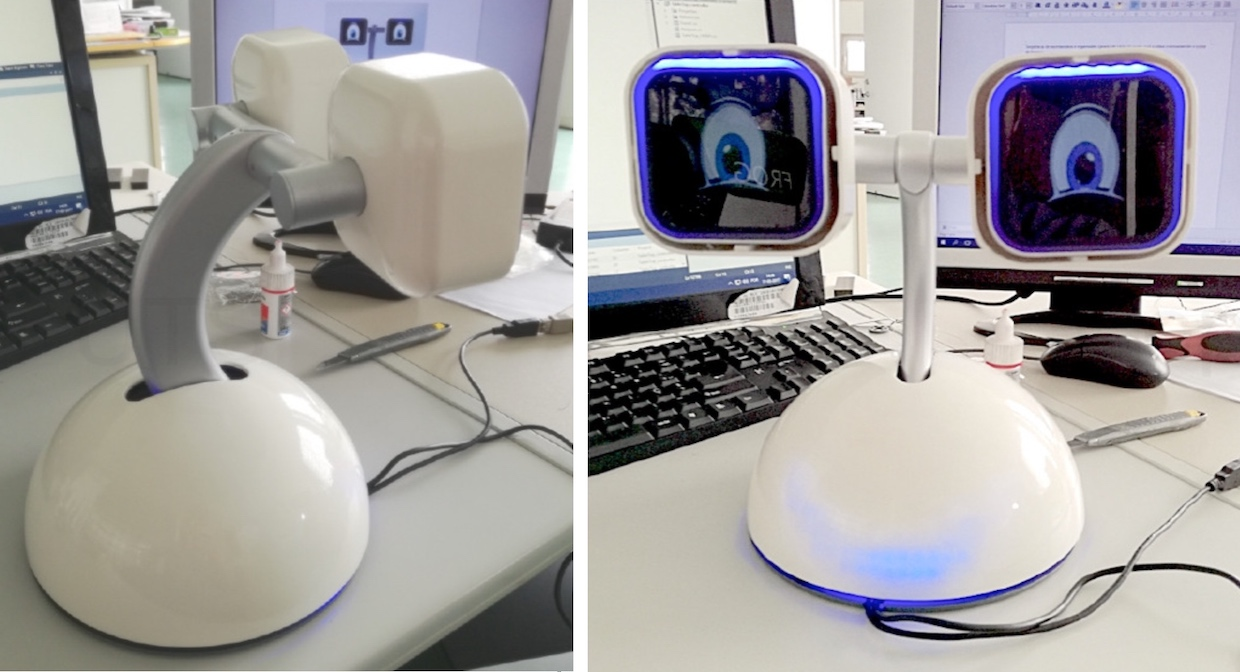
\includegraphics[width=\linewidth]{mirage/haru.jpeg}
    \captionof{figure}{The Haru Robot.}
    \label{fig:mirage:haru}
}
In particular, the method was tested on an autonomous robot platform called \library{Haru}\citeonly{ackerman2018haru, gomez2018haru}, consisting of a base and two screens mimicking a face with two eyes (See~\cref{fig:mirage:haru})
The robot will be fitted with actuators (for the whole body, the neck, and the eyes) and cameras and a microphones for visual and auditory sensing.
The partner agreed on using its technology to see the impact of echo-aware sound source localization.
Therefore, the multichannel extention of this method consider the circular microphone array featuring 7 sensor of the \library{Haru} robot.
The results of this study was described in an internal technical report~\citeonly{di2019honda}.


\section{Literature review in Echo-aware Sound Source Localization}
Common to most sound source localization approaches reviewed in ~\cref{subsec:application:localization} is the challenge posed by environment reverberation.
It is typical to observe that \ac{DOAs} estimation degrades with increasing acoustic reflection~\citeonly{chen2006time}.
For these reasons, most sound source localization methods regard reverberation and, in particular, acoustic echoes as a nuisance.
Room reverberation is considered in the works~\citeonly{rui2004time, chen2006time, zhang2007maximum} while the authors of~\citeonly{weinstein1994iterative, taghizadeh2015spatial, salvati2016sound} attempt to solve \SSL/ by estimating the full \RIRs/.
However, both the cases have drawbacks: in the former, the generic model for reverberation does not reduce strong early echoes, and in the latter, \RIRs/ estimation is a difficult task.

\mynewline
The echo-aware sound source localization methods take another direction: they exploit the closed-form relation between echoes timings and audio scene geometry expressed by the \ISMdef/.
Early works such as~\citeonly{korhonen2008acoustic, ribeiro2010turning, ribeiro2010using, svaizer2011use} uses knowledge form the room geometry to estimated the position of the sound source with respect to the arrays.
This idea was subsequently extended in later works, reducing the amount of prior knowledge required or addressing different applications.
The authors of \citeonly{nakashima2010localization}  study the \SSL/ problem in binaural recordings.
To improve localization, they propose to used ad-hoc reflectors as artificial \textit{pinnae} and a simple reflection model.
In the work~\citeonly{krekovic2016echoslam}, the author addresses the problem \ac{SLAM}\sidenote{
    \ac{SLAM} enables the estimation of a moving robot’s position in relation to a number of external acoustic sources.
} using echoes.
The authors of~\citeonly{an2018reflection} propose to use cameras, depth sensors, and laser sensors to identify reflectors and build a corresponding acoustic model that is used
for echo-aware \ac{SSL}.
Finally, in a very recent work, the well-known \ac{MUSIC} framework for localizing multiple sources is modified for accounting an echo model for the spherical harmonic representation~\citeonly{birnie2020reflection}

\mynewline
All the above mentioned echo-aware methods are explicitly knowledge-driven, namely, using closed-form solutions based on physics, acoustics, and signal processing models.
As explained in the previous chapter, data-driven methods, especially \ac{DNN}, have been successfully applied to address \SSL/.
The main benefit is in their ability to learn complex mapping functions based on simple input-output pairs.
However, they are typically trained for specific applications and use-cases (\eg/, arrays geometry, acoustic conditions, \etc/) and fail whenever test conditions strongly mismatch training conditions.

\section{Proposed Approach}
In the work \cite{di2019mirage}, we proposed to combine the best of the two worlds:
using a deep learning model to estimate challenging acoustic parameters and a physically-motivated model to map such parameters to source's \DOAs/.
To this end, we introduce the framework of \MIRAGEdef/ for \SSL/, based on the \textit{image microphones} model~\citeonly{bergamo2004collaborative,korhonen2008acoustic} (See~\cref{sec:separake:sota}).

\mynewline
Let us consider a simple yet common scenario to illustrate this idea:
two microphones, one source, and a nearby reflective surface, as illustrated in Fig. \cref{fig:mirage:scene}.
\marginpar{%
    \centering
    \footnotesize
    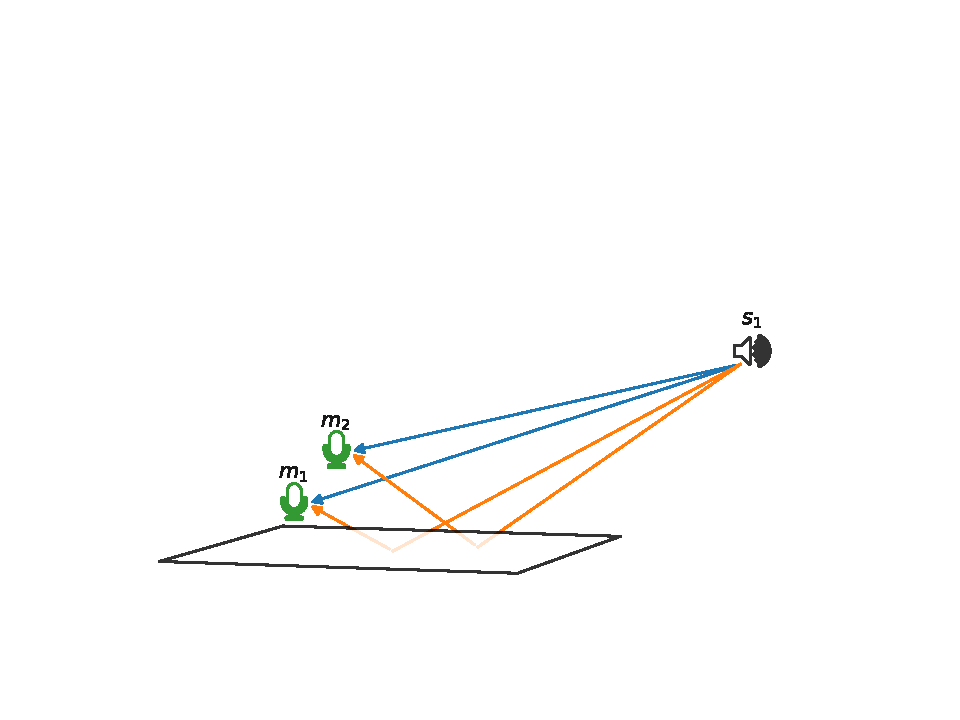
\includegraphics[trim={50 70 50 150},clip,width=\linewidth]{mirage/scene.pdf}
    \captionof{figure}{%
        Typical setup with one source source recorded by two microphones.
        The illustration shows direct sound path (blue lines) and resulting first-order echoes (orange lines).}
    \label{fig:mirage:scene}
}
This may occur when the sensors are placed on a table or next to a wall.
Striking examples of these scenarios are the smart table-top devices, such as Amazon Echo, Google Home, \etc/.
The reflective surface is assumed to be the most reflective and closest one to the microphones in the environment, generating the strongest and earliest echo in each microphone.
Under this stereophonic \textit{close-surface} model, we ask the following questions.

\questionpar{Can early echoes be estimated from two-microphone recordings of an unknown source?}
This question was already addressed in~\cref{pt:estimation}.
In particular, we proposed to use the \ac{DNN} models discussed in~\cref{ch:lantern}.
The models are trained on a simulated close-surface dataset to estimate early echoes properties from audio features.

\questionpar{Can early echoes be used to estimate both the azimuth and elevation angles of the source?}
Note that this is considered as an \textit{impossible} task in free field stereophonic conditions.
To answer the second question, we propose the \ac{MIRAGE} framework.
It exploits echoes' time of arrival by expressing them as \acp{TDOA} in the \textit{virtual 4-microphone array} formed by the true microphone pair and its image with respect to the reflective surface.
We show that this framework approximately estimates echo properties, perform similarly to a correlation-based method in azimuth estimation for the considered
scenario and estimates \textit{impossible} elevation angles with good accuracy in noiseless settings using two microphones only.


\section{Background in microphone array SSL}\label{sec:background}
In this section, we briefly review some necessary background in microphone array \ac{SSL}.
Let us assume a microphone array of $\idxMic$ sensors is placed inside a room and records the sound emitted by one static point sound source ($\numSrcs=1$).
In all generality, the relationship between the signal $\mic_\idxMic$ recorded by the $\idxMic$-th sensor placed at fixed position $\positionMicrophone_\idxMic$ and the signal $\src$ emitted by the source at fixed position $\positionSource$ is defined by:
\begin{equation}\label{eq:mirage:anymic_time}
\mic_i[n] = (\flt_\idxMic \convDis \src)[n]  \; + \; \nse_\idxMic[n],
\end{equation}
where the convolution with \RIR/ $\flt_\idxMic[n]$ embodies the fact that sensor $\idxMic$ receives a spatial image of the source and $\nse_\idxMic$ denotes possible measurement noise.
As fully described in~\cref{ch:acoustic}, the \RIR/ depends on the spatial parameters of the scene: microphone positions, source position \wrt/ the room, as well as the room acoustic properties (size, absorption, and diffuseness of the wall materials).

\mynewline
Let us assume that \RIRs/ follows the echo model under the narrowband approximation presented in~\cref{subsec:processing:stft}.
Therefore, in the discrete-frequency domain, this leads to
\begin{equation}\label{eq:mirage:rir}
    \FLT_\idxMic[k] = \sum_{\idxEch=0}^{\numEchs}  \; \alpha_\idxMic^{(\idxEch)}[k] \; \cste^{- \csti 2 \pi f_k \tau_\idxMic^{(\idxEch)}} \; + \; \varepsilon_\idxMic[k],
\end{equation}
where $f_k$ is the $k$-th frequency bin and the error term $\varepsilon_i[k]$ collects later echoes, the reverberation tail, diffusion, and noise.
In this work, we will consider only the first strongest echo, therefore $R = 1$.
Note that for $r=0$ denotes the ideal propagation path,
being $\tau^{(0)_\idxMic}$ the ideal propagation path from the source to the $\idxMic$-th microphone, and $\alpha^{(0)_\idxMic}$ the air attenuation.
In the remainder of this work, we make the approximation of $\alpha_i^{(\idxEch)}$ being frequency-independent.

\subsection{2-channel 1D-SSL}\label{subsec:mirage:1D-SSL}
\newcommand{\tdoa}{\ensuremath{\tau_\mathtt{TDOA}}}
\newcommand{\aoa}{\ensuremath{\vartheta}}
Let us first consider the case of stereophonic recordings ($\numMics=2$).
Under the far- and free-field assumption, traditional \SSL/ methods use the \acf{TDOA},
\begin{equation*}
    \tdoa \eqdef \tau^{(0)}_2 - \tau^{(0)}_1\quad\text{[second]}
    ,
\end{equation*}
as a proxy for the estimation of the \ac{AOA}, $\aoa$, since:
\begin{equation}\label{eq:mirage:aoa}
    \vartheta = \arccos \kparen{\speedOfSound \: \tdoa \: / \: \distMicMic }\quad\text{[rad]},
\end{equation}
where $\speedOfSound$ is the speed of sound and $\distMicMic$ the inter-microphone distance.

\begin{figure}
    \begin{sidecaption}[]{
        Illustration of the relation between \ac{DOA} and \ac{TDOA} with ones source and two microphone.
        Knowing the distance $\distMicMic$ between the two microphones, simple trigonometry yields the \ac{AOA} $\vartheta$ according to~\cref{eq:mirage:aoa}.
    }[fig:mirage:gcc]
        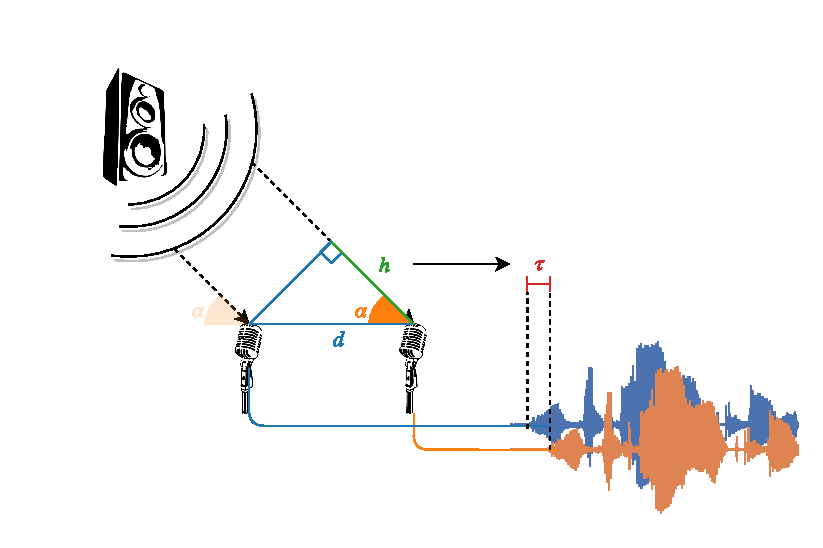
\includegraphics[width=\linewidth]{mirage/tdoa_microphone.pdf}
    \end{sidecaption}
\end{figure}


\mynewline
Then, \SSL/ reduces to estimating the \ac{TDOA}, which can be done by \ac{CC}-based methods such as the widely used and well performing \ac{GCC-PHAT} method \citeonly{knapp1976generalized, blandin2012multi}.
Given \STFT/ $\MIC_1$ and $\MIC_2$ of the two microphones signals, the \ac{CC} and \ac{GCC-PHAT} \textit{angular spectra} are defined as:\marginpar{
    \footnotesize\itshape
    The ``generalized'' cross-correlation methods adds weighting functions (\eg/ the phase transfor (PHAT),  or the smoothed coherence transform (SCOT))
    to the \ac{CC}. Their purpose is to improve the estimation of the time delay on specific characteristic of the signal and noise.
    See~\citeonly{chen2006time} for an overview.
}
\begin{equation}\label{eq:mirage:cc}
    \Psi_\mathtt{CC}(\tau) = \sum_{k,l} \MIC_1[k,l] \khermitian{\MIC}_2[k,l] \cste^{-\csti 2  \pi f_k \tau}
    ,
    \end{equation}
\begin{equation}\label{eq:mirage:gccphat}
    \Psi_\mathtt{PHAT}(\tau) = \sum_{k,l}\frac{\MIC_1[k,l] \khermitian{\MIC}_2[k,l]}{\kvbar{ \MIC_1[k,l] \khermitian{\MIC}_2[k,l] }} \cste^{-\csti 2  \pi f_k \tau}
    ,
\end{equation}
where $\kvbar{\cdot}$ denotes the absolute value and the weighting function $1 / \kvbar{ \MIC_1[k,l] \khermitian{\MIC}_2[k,l]}$ is called \textit{phase transform},
aiming at reducing the source's autocorrelation component from the angular spectrum.

\mynewline
Then, the \ac{TDOA} estimate is given by
\begin{equation*}
    \hat{\tau}_\mathtt{TDOA} = \arg \underset{\tau}{\max} \; \Psi(\tau)
    ,
\end{equation*}
with $\Psi$ begin either $\Psi_\mathtt{CC}(\tau)$ or $\Psi_\mathtt{PHAT}(\tau)$.
Note that these functions can also be expressed directly as a function of the \ac{AOA} using \eqref{eq:mirage:aoa}, hence the term \textit{angular spectrum}.
Despite the theoretical limits of this method, discussed in~\citeonly{chen2006time}, this method is known to work well in practice.
Moreover, it was showed to be state-of-the-art for \ac{SSL} in a large benchmark study~\citeonly{blandin2012multi}.

\subsection{Multichannel 2D-SSL}\label{subsec:mirage:2D-SSL}
When more microphones are available and the microphones array is compact and not linear\sidenote{
    In case of complanarity, the angle can be estimated up to ``up-down'' umbigity.
}, 2D-\ac{SSL} can be envisioned
A possible approach is to use 1D-\ac{SSL} on all pairs and combine their results, a principle which was successfully applied in the \acf{SRP-PHAT} method \citeonly{dibiase2001robust}.


\mynewline
\begin{figure}
    \begin{sidecaption}[t]{
        Illustration of the different \acp{DOA} at each microphone pairs listening one sound source.
        Knowing the position of the microphone, the angle with respect to a reference point can be deduced in closed-form.
    }[fig:mirage:gcc]
        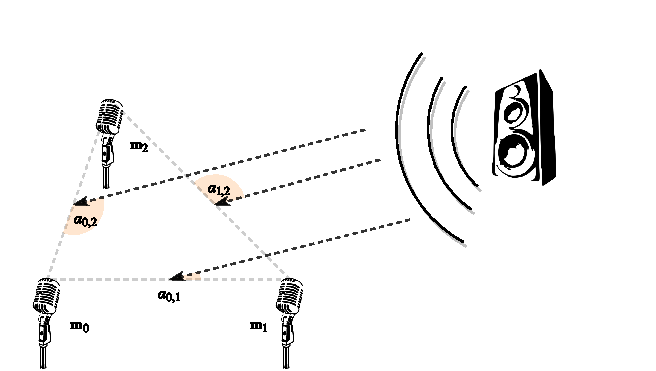
\includegraphics[width=\linewidth]{mirage/srp-phat_aggregation.pdf}
    \end{sidecaption}
\end{figure}
The \ac{SRP-PHAT} methods returns the source's \ac{DOA}, namely the pair azimuth and elevation $(\theta, \phi)$, by estimating \acp{TDOA} from each microphone pairs.
In order to achieve this, it requires the geometry of the microphone array to be known.
In a nutshell, this algorithm aims to estimate a \textit{global angular spectrum} $\Psi_{\mathtt{SRP}}(\theta,\phi)$ in the polar coordinates system with respect to reference point in the array, typically its barycenter.
This function will exhibit a local maximum in the direction of the active source.
\\The algorithmic can be exemplified in the following steps:\marginpar{
    \footnotesize\itshape
    See \href{http://bass-db.gforge.inria.fr/bss_locate/}{\library{MBSSLocate} \ExternalLink} for a free MATLAB implementation and comprehensive documentation of this algorithm.
}
\begin{enumerate}
    \item a global grid of \acp{DOA} candidates is defined according to a desired resolution and computational load;
    \item for each pair of microphones, a local set of \ac{AOA} (hence, \acp{TDOA}) is defined based on the above chosen \acp{DOA} and the input geometry;
    \item a TDOA-based algorithm (\eg/ \ac{GCC-PHAT}) is used to compute the associated local angular spectrum;
    \item all the local contributions (a collection of local $\Psi_\mathtt{GCC}(\tau)$) are geometrical aggregated and interpolated back to the global \ac{DOA} grid to form $\Psi_{\mathtt{SRP}}(\theta,\phi)$;
    \item the \acs{DOA}(s) maximizing $\Psi_\mathtt{SRP}$ is (are) used as estimate (in case of multiple sources).
\end{enumerate}
This algorithm can be seen as an application of the divide-and-conquer paradigm to \ac{TDOA}-based methods:
``at the leaves'', the \ac{GCC-PHAT} method provide \ac{TDOA} for each microphone pair;
the ``merge'' operation consists in aggregating \ac{TDOA} defined on a different axis based on the knowledge of the array geometry.
Finally, we stress that this algorithm is independent of the method used to estimate the \ac{TDOA}.

\section{Microphone Array Augmentation with Echoes}\label{sec:mirage:mirage}
We now introduce the proposed concept of \MIRAGEdef/.
Eq.~\cref{eq:mirage:echo_h} then corresponds to the well known \acf{ISM}, where reflections are treated as mirror images of the true source with respect to reflective surfaces, emitting the same signal.
\marginpar{%
\centering
\footnotesize
    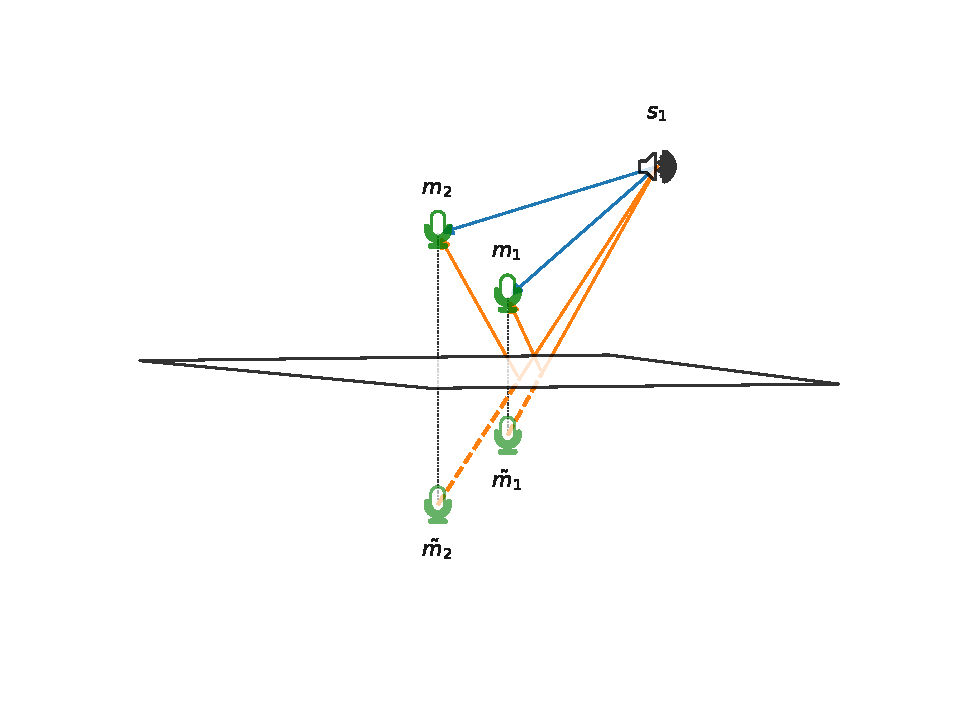
\includegraphics[trim={90 75 40 50},clip,width=\linewidth]{mirage/mirage.pdf}
    \captionof{figure}{%
        Illustration of the images $\mathring{\positionMicrophone}_1$ and $\mathring{\positionMicrophone}_2$ of microphones $\positionMicrophone_1$ and $\positionMicrophone_2$ in the presence of a reflective surface and a source.
        Blue lines correspond to direct paths, orange lines correspond to echo paths.}
    \label{fig:mirage:mirage}
}
We will employ here a less common but equivalent interpretation of \ISM/, namely, the image-microphone (IM) model. As illustrated in Fig.~\cref{fig:mirage:mirage}, virtual microphones are mirror images of the true microphones with respect to reflective surfaces.
In this view, the echoic signal received at a true microphone is the sum of the anechoic signals received at this microphone and its images.
If we consider the virtual array consisting of both true and image microphones, multiple microphone pairs are now available. For each of them, it is then possible to define a corresponding time difference of arrival.
Among them, we will refer to the one between the two real microphones as \ac{TDOA}, the one between the two image microphones as \ac{iTDOA} and the one between the first microphone and its image as \ac{TDOE}.
Therefore, we have:\marginpar{%
    \centering
    \footnotesize
    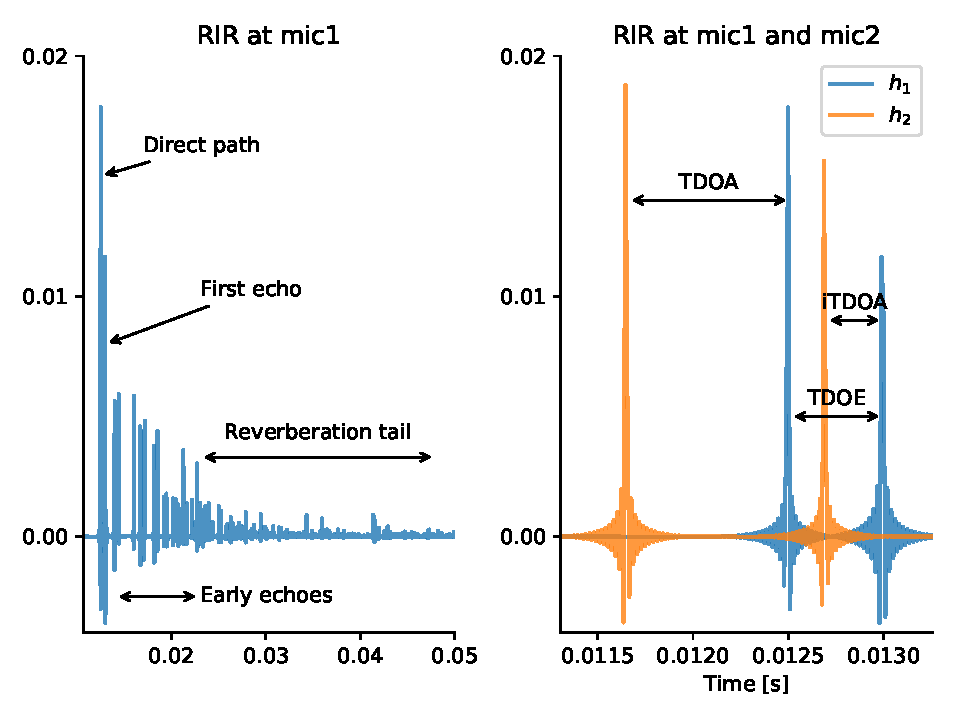
\includegraphics[trim={82mm 0 0 0},clip,width=\linewidth,height=7cm]{mirage/rirs.pdf}
    \captionof{figure}{%
        Superposition of two \acp{RIR} and visualization of time difference of arrival between direct paths (\ac{TDOA}), first echoes (\ac{iTDOA}) and direct path and first echo (\ac{TDOE}).}
    \label{fig:mirage:rirs_tdoa}
}%
\begin{align}
\tau_\mathtt{TDOA}  &= \tfrac{1}{c} \norm{\positionMicrophone_2 - \positionSource} - \tfrac{1}{c} \norm{\positionMicrophone_1 - \positionSource} = \tau_2^{(0)} - \tau_1^{(0)},\\
\tau_\mathtt{iTDOA} &= \tfrac{1}{c} \norm{\mathring{\positionMicrophone}_2 - \positionSource} - \tfrac{1}{c} \norm{\mathring{\positionMicrophone}_1 - \positionSource} = \tau_2^{(1)} - \tau_1^{(1)},\\
\tau_{\mathtt{TDOE},1}  &= \tfrac{1}{c} \norm{\mathring{\positionMicrophone}_1 - \positionSource} - \tfrac{1}{c} \norm{\positionMicrophone_1 - \positionSource} = \tau_1^{(1)} - \tau_1^{(0)}\\
\end{align}
where $\mathring{\positionMicrophone}_i$ denotes the position of the image of $\positionMicrophone_i$ with respect to the reflector.
Note that $\tau_{\mathtt{TDOE},2} = \tau_\mathtt{iTDOA} + \tau_{\mathtt{TDOE}, 1} - \tau_\mathtt{TDOA}$.
These three quantities are directly connected to \RIRs/, as illustrated in~\cref{fig:mirage:rirs_tdoa} (Right).
Let $V = \set{\tau_{\mathtt{TDOA}}, \tau_{\mathtt{iTDOA}}, \tau_{\mathtt{TDOE},1}}\in\mathbb{R}^3$


\mynewline
Following the 2D-\SSL/ scheme described in \cref{subsec:mirage:2D-SSL} and given the virtual microphone-array geometry (which depends on the relative position of microphones to the surface),
$V$ could in principle be used to estimate the 2D directional of arrival of the source.
In the~\cref{ch:lantern}, we introduced a learning-based method to estimate $V$ using audio features obtained from only two microphones.

\mynewline
As stated is section \ref{subsec:mirage:2D-SSL}, given a microphone pair, the peak of angular spectrum $\Psi_\text{PHAT}$ corresponds to the \ac{TDOA}.
Moreover, peaks corresponding to the early reflection are presents.
\cref{fig:mirage:noise_ang_spec} shows the $\Psi_\mathtt{CC}$'s and the $\Psi_\mathtt{PHAT}$'s angular spectra for synthetic data where the source signal is noise or speech for all the pairs of the HARU's circular microphone array.
The location of the quantities in $V$ are highlighted with vertical dotted lines.
Theoretically, when only the first reflection are considered ($K=1$), the position of the peaks in the angular spectra correspond to
$\tau_\mathtt{TDOA}$, $\tau_\mathtt{iTDOA}$, $\tau_\mathtt{TDOA} - \tau_{\mathtt{TDOE}, 1}$, and $\tau_\mathtt{TDOA} + \tau_{\mathtt{TDOE}, 2}$.
It is important to note that for speech signals, $\Psi_\text{PHAT}$ removes the auto-correlation part in order to promote a sharp peak at the position of the \ac{TDOA}.
Since acoustic echoes increase the auto-correlations of the signal in one microphones, the \ac{PHAT} transform tends to lower their contribution, so that their peaks are not distinguishable from spurious ones.
\begin{figure}
    \begin{fullwidth}
        \centering
        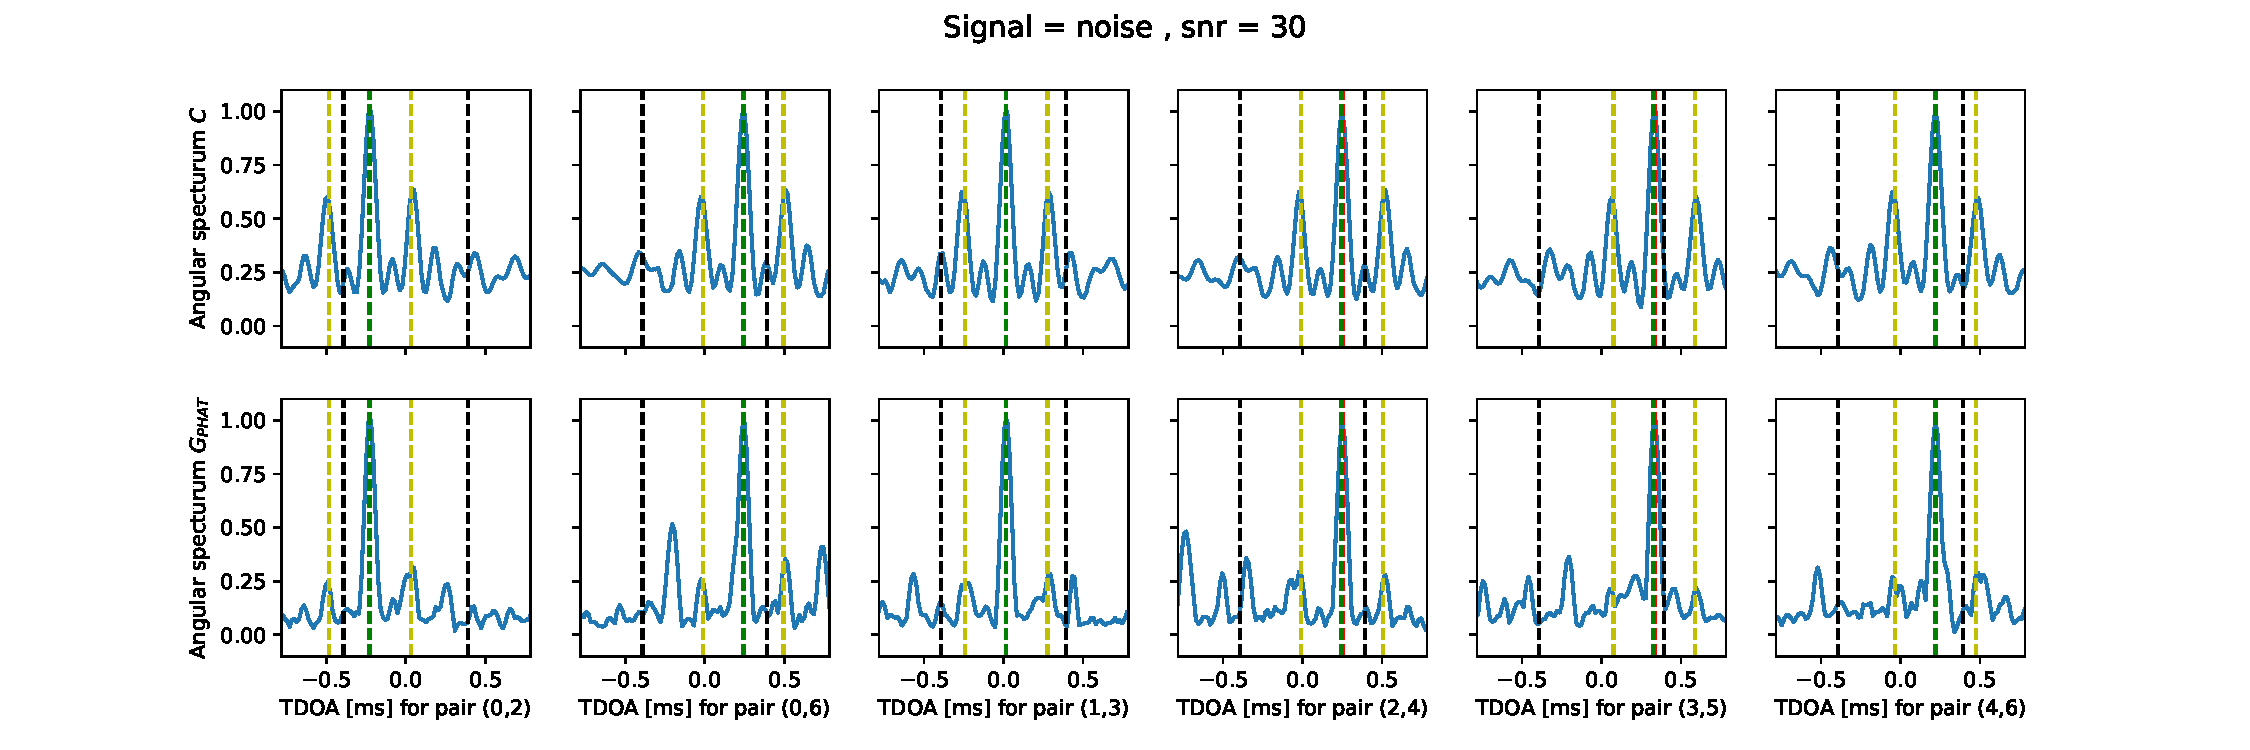
\includegraphics[trim={0mm 0 0mm 0},clip,width=\linewidth]{mirage/echo_hunting_broadband.pdf}
        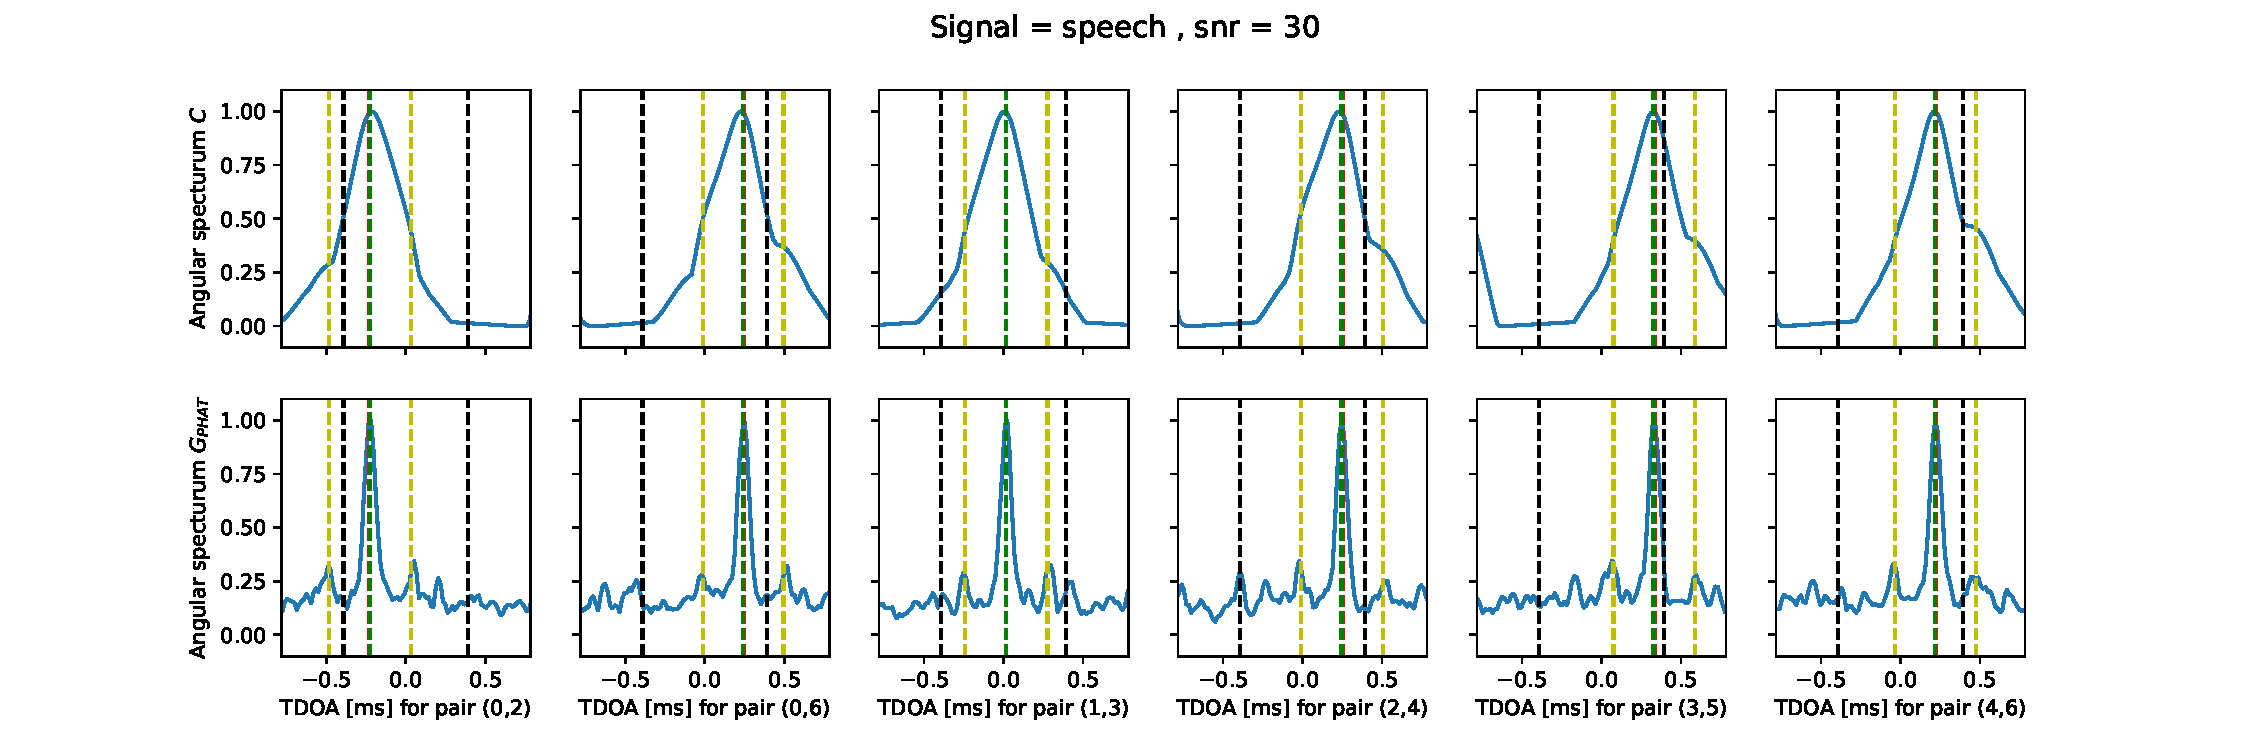
\includegraphics[trim={0mm 0 0mm 0},clip,width=\linewidth]{mirage/echo_hunting_speech.pdf}
        \caption{
            Angular Spectra $\Psi_\mathtt{CC}$ and $\Psi_\texttt{PHAT}$ for different pairs of microphone in the HARU array using synthetic \RIRs/ and \textit{white noise} (top) and \textit{speech} (botton) signal .
            Vertical lines mark the positions of  $\tau_\mathtt{TDOA}$ (red), $\tau_\mathtt{iTDOA}$ (green), $\tau_\mathtt{TDOA}-\tau_\mathtt{TDOE,1}$ (yellow) and $\tau_\mathtt{TDOA}+\tau_\mathtt{TDOE,2}$ (yellow) are marked with vertical lines.
            The black vertical lines correspond to the maximum TDOA given the pair distance, \textit{i.e.} corresponding to the AOA $ = \{0, 2\pi\}$}
        \label{fig:mirag:noise_ang_spec}
    \end{fullwidth}
\end{figure}


\section{Experimental Results}\label{sec:mirage:exp}

\subsection{2-channel scenario}
To the best of the authors' knowledge, no reference implementation of algorithms for 2D-SSL using only 2 microphones is available to date.
To check the validity of \ac{TDOA}s estimation, our approach is compared to \ac{GCC-PHAT} using only the true microphones (see Sec. \cref{subsec:mirage:1D-SSL}).

\mynewline
The \ac{DNN} model is trained and validated on many random, shoe-box room configurations generated by the software presented in \citeonly{schimmel2009fast}.
This software implements both the image-method for simulating reflections and a ray-tracing algorithm for diffusion.
Room widths are uniformly drawn at random in $[3, 9]$~m, heights in $[2, 4]$~m.
Random source/microphones positions and absorption coefficients for the 6 surfaces are used,
respecting the close-surface scenario. In particular, the microphones are at most $30$ cm from the close-surface,
placed $10$ cm from each other, the absorption coefficients of the other walls are
uniformly sampled in $(0.5, 1)$ and the one of the close-surface is in $(0, 0.5)$.
The same realistic diffusion profile \citeonly{gaultier2017vast} is used for all surfaces.
Around $90,000$ audio scenes are generated this way, yielding reverberation time \RT{} between $20$~ms and $250$~ms.

\mynewline
For both training and validation, the \acp{RIR} are convolved with 1~second of white-noise (wn) with no additional noise.
All signals and RIRs are sampled at $\SI{16}{kHz}$.
The \STFT/ is performed on 1024 point with 50\% overlap.
Finally, the features are computed as in~\eqref{eq:mirage:features} yielding a vector of size $D = 1534$ for each observation.
While we validate the MLP on a portion of the dataset in a \textit{holdout} fashion, the test is conducted on 200 new \acp{RIR} convolved with both wn and speech (sp) utterances.
This set is generated similarly to the training and validation sets. Moreover the recordings are perturbed by external white noise at 10 dB SNR (wn+n, sp+n).
The speech signals are normalized speech utterances of various lengths (from $1$ s to $6$ s), randomly selected from the TIMIT corpus.
A free and open-source Matlab implementation of \ac{SRP-PHAT}\sidenote{\href{http://bass-db.gforge.inria.fr/bss_locate/}{MBSSLocate \ExternalLink}} is used to aggregate local angular spectra obtained from the \ac{DNN}'s output.
The same toolbox is used for the implementation of \ac{SRP-PHAT} with \ac{GCC-PHAT}.
For the latter method only real pairs are used.
A sphere sampling with $\ang{0.5}$ resolution and coordinates $\theta \in [-179, 180]$ and $\phi \in [0, 90]$ is used for the \c{DOA} search.


\begin{table}[ht]
\begin{sidecaption}[DoA estimation]{%
    Mean angular error in degree (with accuracies ($\%$)) for 2D SSL (azimuth and elevation)
    with $\ang{10}$ and $\ang{20}$ tolerance.}[tab:mirage:doa]
    \small
    \centering
    \begin{tabular*}{\linewidth}{@{\extracolsep{\fill}}cl|cc|cc@{}}
    \toprule
    \ac{DOA}        &            &  \multicolumn{2}{c|}{ACCURACY}    &   \multicolumn{2}{c}{ACCURACY} \\
                    &            &  \multicolumn{2}{c|}{$<\ang{10}$} &   \multicolumn{2}{c}{$<\ang{20}$} \\
                    &    Input   &  $\theta$ &  $\phi$ &  $\theta$ &  $\phi$ \\
    \midrule
    MIRAGE &  wn    &   4.5 (59) &  3.9 (71) &   6.8 (79) &   5.9 (88) \\
    MIRAGE &  wn+n  &   4.4 (18) &  5.5 (26) &   9.4 (35) &  11.1 (66) \\
    MIRAGE &  sp    &   4.6 (45) &  4.8 (59) &   8.1 (71) &   7.2 (83) \\
    MIRAGE &  sp+n  &   5.2 (17) &  5.9 (12) &  10.7 (38) &  12.3 (43) \\
    \bottomrule
    \end{tabular*}
\end{sidecaption}
\end{table}

\mynewline
\ac{TDOA} estimation errors using the proposed approach and \ac{GCC-PHAT} are presented in Table~\cref{tab:mirage:tdoas-aoa}.
Training a \ac{DNN} to estimate \acp{TDOA} brings similar performances as \ac{GCC-PHAT} in terms of \ac{nRMSE}.
Estimation of \acp{iTDOA} and \ac{TDOE} seems to be a harder task for the simple \ac{DNN} we used.
Nevertheless, our results confirm the possibility of retrieving early echoes from only two-microphone recordings.
When some external noise is added, performance of both methods severely degrades.
This is a well-know and expected behavior for \ac{GCC-PHAT}.
It suggests that noise should be considered in the training phase of \MIRAGE/.
When we compare the performance in terms of \ac{AOA}, the two methods yield the same accuracy within a $\ang{20}$ threshold, as can be see in Table~\cref{tab:mirage:tdoas-aoa}.
When a smaller tolerance is considered, GCC-PHAT outdoes the proposed approach in accuracy, with comparable errors.
This behavior is due to two aspects: first, the synthetic angular spectrum is might be a too simple model; second, since \ac{nRMSE} was chosen as validation metrics, accuracy is not directly optimized.
Again, when adding noise, performance decreases.

\mynewline
In Table~\cref{tab:mirage:doa} the performance of the full 2D-SSL pipeline is showed.
Within a tolerance of $\ang{20}$, the \MIRAGE/ model allows estimation of both azimuth and elevation of the target source.
However since in our data the 2 microphones were free to move, the inclinations of the true and image pairs are rarely flat.
While this helps elevation estimation, it reduces the accuracy of predicting the right azimuth.
While external noise is again decreasing the accuracy dramatically,
it is interesting to notice that our \ac{DNN} model trained and validated with white noise sources somewhat generalizes to speech sources.

\mynewline
In this paper we demonstrated how a simple echo model could allow 2D SSL with only two microphones, using simulated data.
Future research will focus on extending this proof-of-concept to real data.
The problem of echo-delay estimation proved to be very challenging, and extensions of the proposed learning scheme will be developed to obtain more reliable estimations of angular spectra.
Extensions of the method to better handle various types of noise and emitted signals will also be sought.
Finally, applications of the MIRAGE framework to larger microphone arrays, higher order echoes and a variety of tasks beyond SSL will be explored.


\subsection{Multi-channel synthetic-data scenario}
In this section, we will compare the \ac{SRP-PHAT} algorithm (using GCC-PHAT for TDOA estimation) with the proposed approach, \MIRAGE/, on multichannel synthetic data generated with the Python library \href{https://github.com/LCAV/pyroomacoustics}\library{pyroomacoustics \ExternalLink}.
The data are created to match the design of the Haru's microphone array placed on top of a table:
the microphones are at most 30~cm from the close-surface, placed $13$ cm from each other; the absorption coefficients of the other walls are uniformly sampled in $(0.5, 1)$ and the one of the close-surface is in $(0, 0.5)$.
In the next paragraph, the two methods are compared for \ac{TDOA} estimation task, while in the following discussion, the performances for 2D-\ac{SSL}.

\newthoughtpar{TDOA estimation on synthetic data}\label{subsec:eval_synth_tdoa}
For this comparison, 200 different audio scenes have been generated, as explained in section~\cref{sec:mirage:exp}.
The following metrics have been used: \ac{nRMSE}, \ac{RMSE} and \ac{STD}.
In~\cref{tab:mirage:tdoa_synth} TDOA estimation errors are presented.
From these results, the proposed approach outperforms the baseline for both speech and noise data.
Even if the \ac{RMSE} of \ac{GCC-PHAT} is lower than \MIRAGE/'s one, the former method produces many more outliers as depicted in~\cref{fig:mirage:tdoa_synth_signals}.
For better understanding, all the error for \ac{TDOA} estimation are computed in samples, that is they are all multiplied by the constant sampling frequency of the signals ($16$~kHz).
As an additional metric, the empirical computational time of the proposed approach is more than 10 times smaller than the baseline.
\begin{table}[h]
    \begin{sidecaption}[]{
        Evaluation metrics (nRMSE, RMSE, STD) for TDOA estimation and empirical computational time for different source signals. In bold the best records.
    }[tab:mirage:tdoa_synth]
        \small
        \centering
        \begin{tabular*}{\linewidth}{@{\extracolsep{\fill}}lllrrrr@{}}
        \toprule
        &           &  signal &     nRMSE &       RMSE &       STD &      time \\
        \midrule
        & MIRAGE      &   noise &  \textbf{0.09} &  0.29 &  \textbf{0.26} &  \textbf{0.19} \\
        & GCC-PHAT    &   noise &  0.26 &  \textbf{0.26} &  1.04 &  2.40 \\
        \midrule
        & MIRAGE      &  speech &  \textbf{0.37} &  \textbf{1.03} &  \textbf{1.09} &  \textbf{0.20} \\
        & GCC-PHAT    &  speech &  0.88 &  2.08 &  2.86 &  2.51 \\
        \bottomrule
    \end{tabular*}
    \end{sidecaption}
\end{table}

\mynewline
In~\cref{fig:mirage:tdoa_synth_snr} the \TDOA/ estimation error is illustrated against the \ac{SNR} level of the recordings.
When the source signal is noise, both methods yield similar mean error independently of the noise level.
However, \ac{GCC-PHAT} seems to produce more outliers lower \ac{SNR}.
On the other hand, when data is speech, for both the approach, the performance decrease as the SNR reduces; however, \MIRAGE/ gives statistically better results in term of standard deviation and outliers.

% \begin{figure}[h]
%     \begin{fullwidth}
%     \centering
%     \subfloat[sinth_data][Synthetic data]{
%         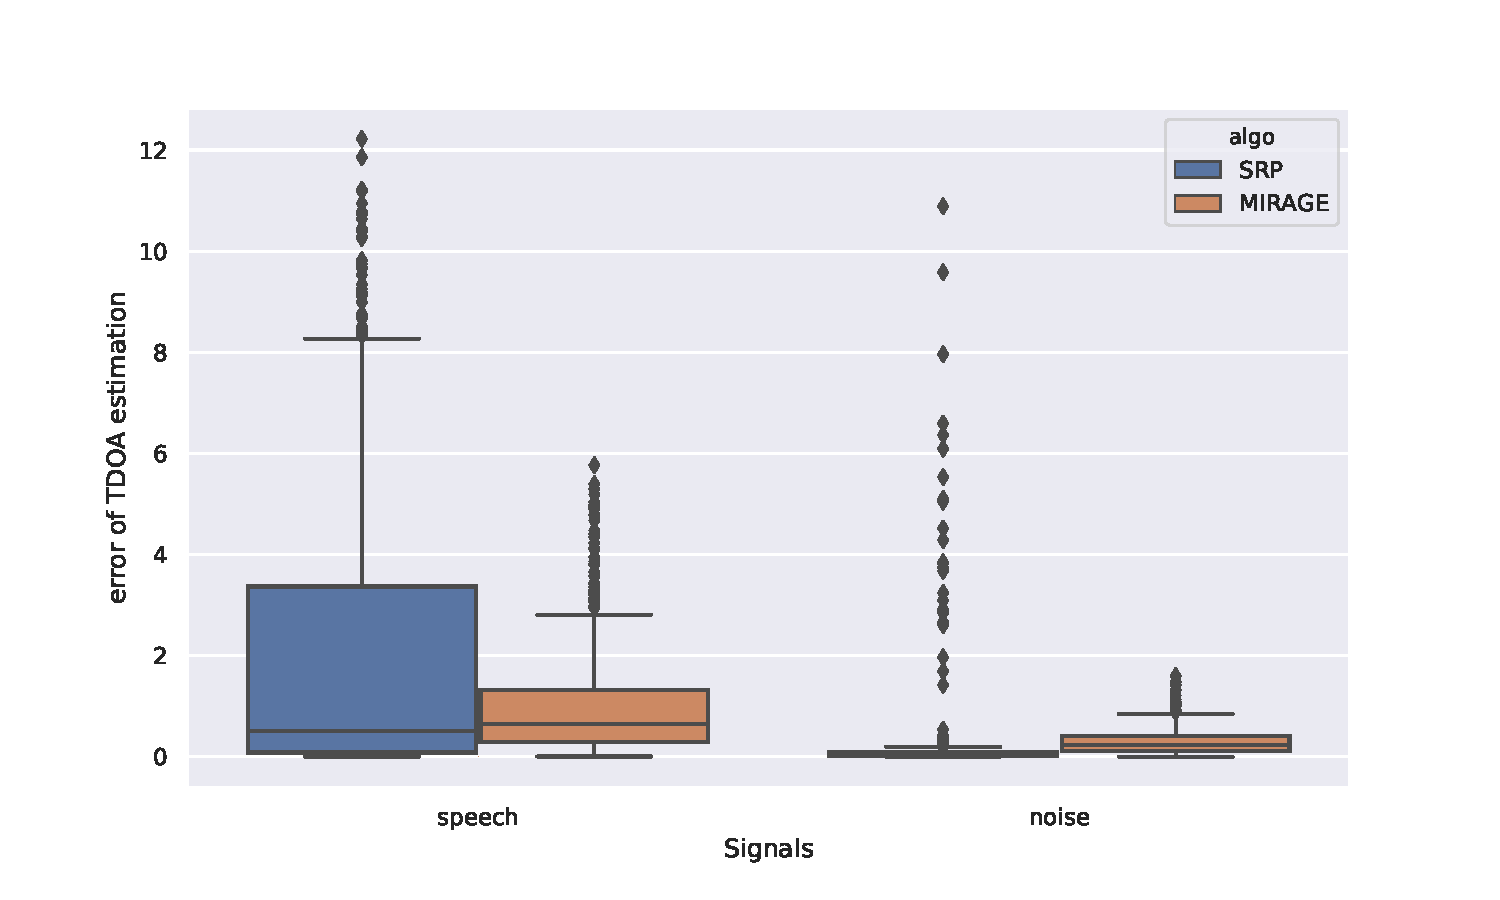
\includegraphics[width=0.48\linewidth]{mirage/box_plot_tdoa_vs_signal.pdf}
%         \label{fig:mirage:tdoa_synth_signals}
%     }
%     \hfill
%     \subfloat[real_data][Real data]{
%         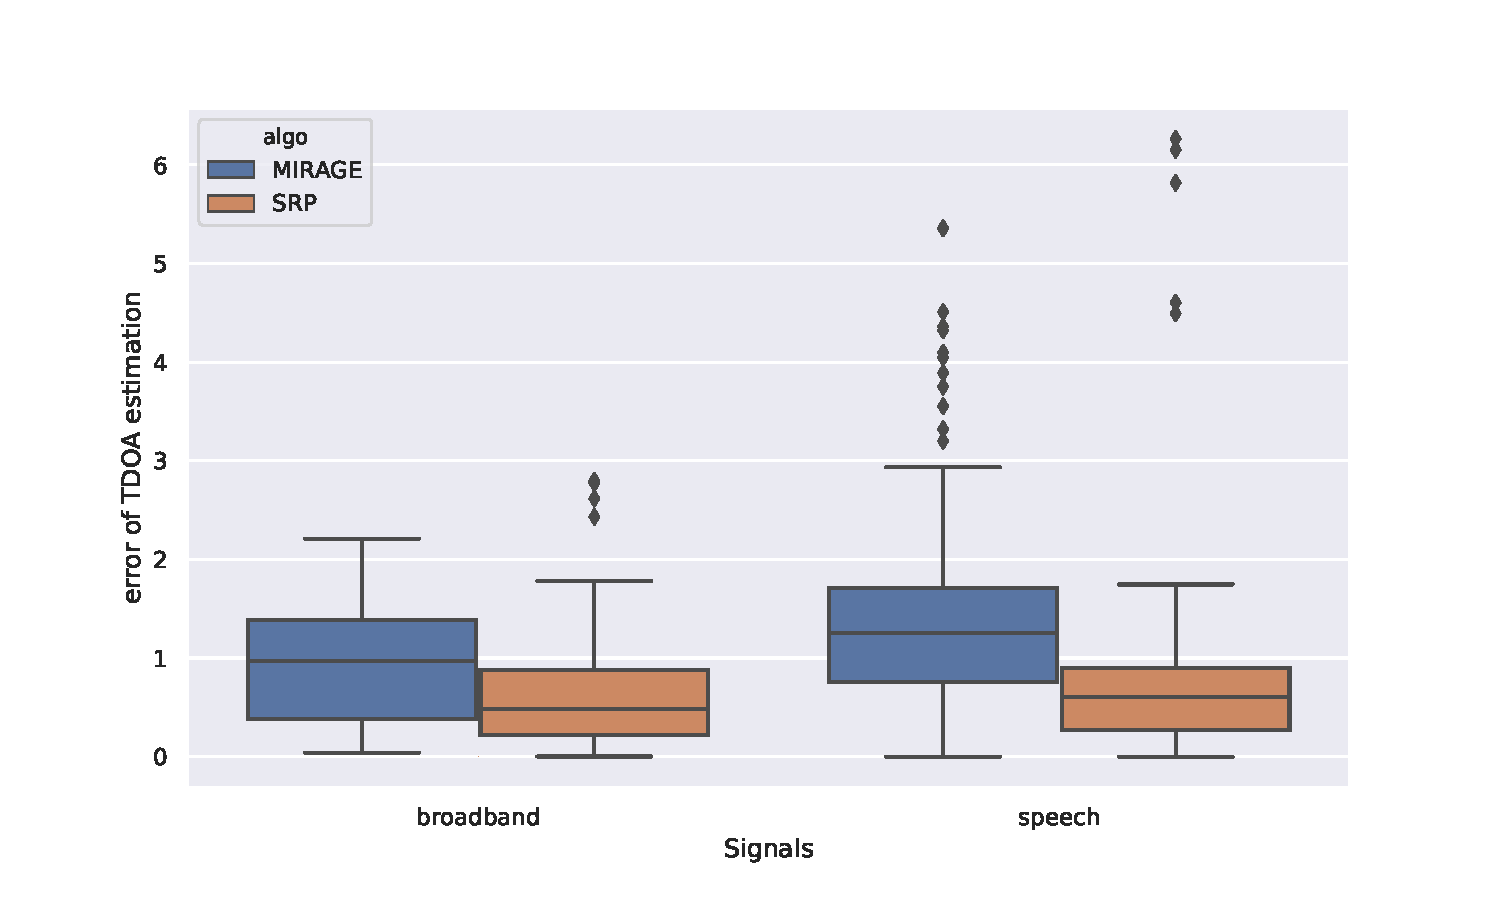
\includegraphics[width=0.48\linewidth]{mirage/box_plot_tdoa_vs_signal_real.pdf}
%         \label{fig:mirage:tdoa_real_signals}
%     }
%     \caption{Box-plots of TDOA estimation errors (in samples) for two different source signals on synthetic data
%             (\cref{fig:mirage:tdoa_synth_signals}) and real data (\cref{fig:mirage:tdoa_real_signals})
%     }
%     \label{fig:mirage:tdoa_signals}
%     \end{fullwidth}
% \end{figure}


\begin{figure}[h]
    \begin{sidecaption}[]{
        Violin-plots of the TDOA errors (in samples) versus SNR ranges (in dB) for speech and noise source signal. Ticks in the SNR axis indicates the upper limit of the following ranges: $(0,5], (5,10], (10,20], (20,30]$ dB.
    }[fig:mirage:tdoa_synth_snr]
    \centering
    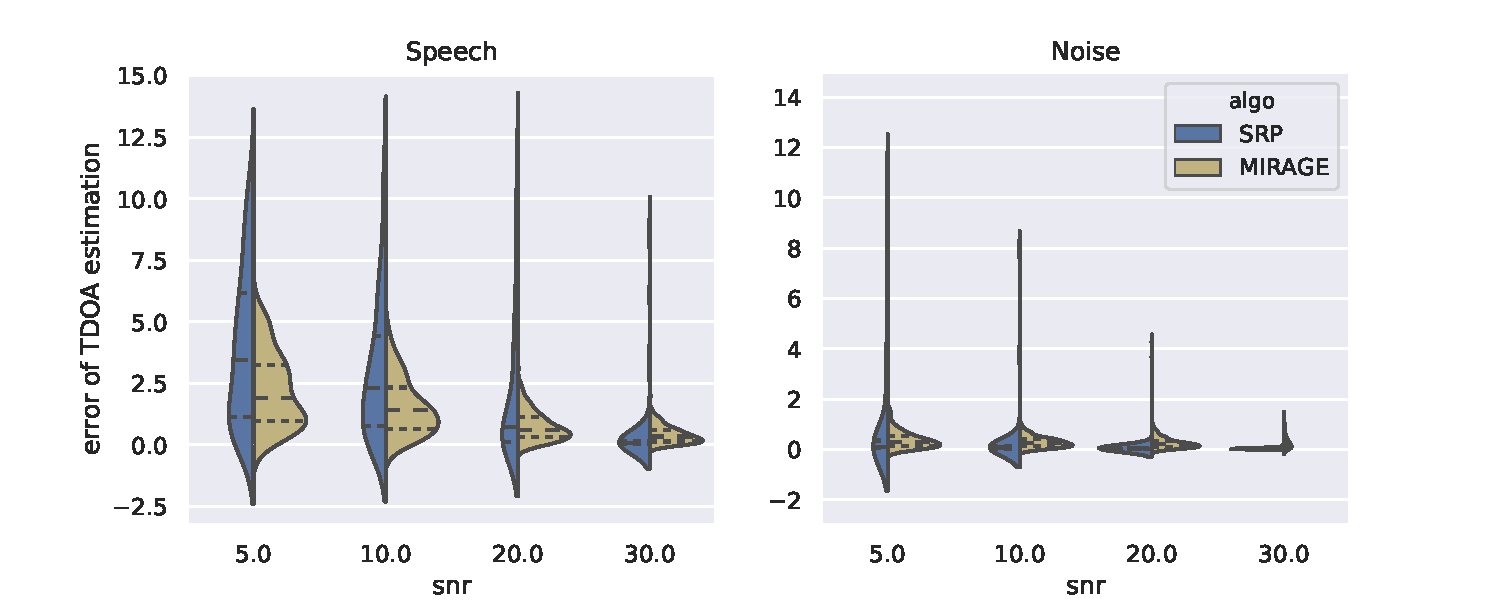
\includegraphics[trim={10 0 5 5},clip,width=\linewidth]{mirage/violinplot_tdoa_vs_snr.pdf}
    \end{sidecaption}
\end{figure}

\newthoughtpar{2D-SSL estimation on synthetic data}
\ac{DOA} estimation errors using the proposed approach and \ac{SRP-PHAT} are presented in~\cref{tab:mirage:ssl_syth}.
For white noise source signals, \ac{SRP-PHAT} has better performances for both elevation and azimuth but with comparable errors.
However, the proposed approach outperforms the baseline when the emitted signal is speech.
\begin{table}[h]
    \begin{sidecaption}[]{
        Mean squared errors and standard deviation in degrees for azimuth ($\theta$) and elevation ($\phi$). In bold the best records.
    }[tab:mirage:ssl_syth]
    \centering
    \small
    \begin{tabular*}{\linewidth}{@{\extracolsep{\fill}}lllllll@{}}
        \toprule
        & &  signal &  Error $\theta$  &  Error $\phi$ \\
        \midrule
        & MIRAGE &   noise &  1.29 $\pm$   1.17 &   2.30 $\pm$   3.35 \\
        & SRP-PHAT &   noise &  \textbf{0.49 $\pm$   0.6}1 &   \textbf{1.70 $\pm$   1.42} \\
        \midrule
        & MIRAGE &  speech & \textbf{ 9.51 $\pm$ 15.84} &  \textbf{12.26  $\pm$  12.20} \\
        & SRP-PHAT &  speech & 35.27 $\pm$  54.57 &  15.10 $\pm$  16.67 \\
        \bottomrule
    \end{tabular*}
    \end{sidecaption}
\end{table}
\\In~\cref{fig:mirage:synth_ssl_noise,fig:mirage:synth_ssl_speech}, the \ac{DOA} estimation results are reported as scatter-plots in a prediction-vs-ground-truth plane.
When the test data contains noise, both the methods perform the same regardless of the \ac{SNR} level.
When speech data are considered, \MIRAGE/ outperforms the baseline, which suffers at a low level of \ac{SNR}.
However, the performance of both of the method drops for elevation estimation.
Unfortunately, this seems to contradict the good performances on \ac{TDOE} estimation, and further investigation is needed to explain this observation.

\begin{figure}[h]
    \begin{sidecaption}[]{
        Scatter-plots (predictions-vs-ground-truth) for DOA estimation (azimuth and elevation) on synthetic data when the the source signal is \textbf{noise}.
        The color map corresponds to different SNR level [dB] in the data.
    }[fig:mirage:synth_ssl_noise]
    \centering
    \subfloat[azel_srp][2D-SSL with SRP-PHAT on noise data]{
        \centering
        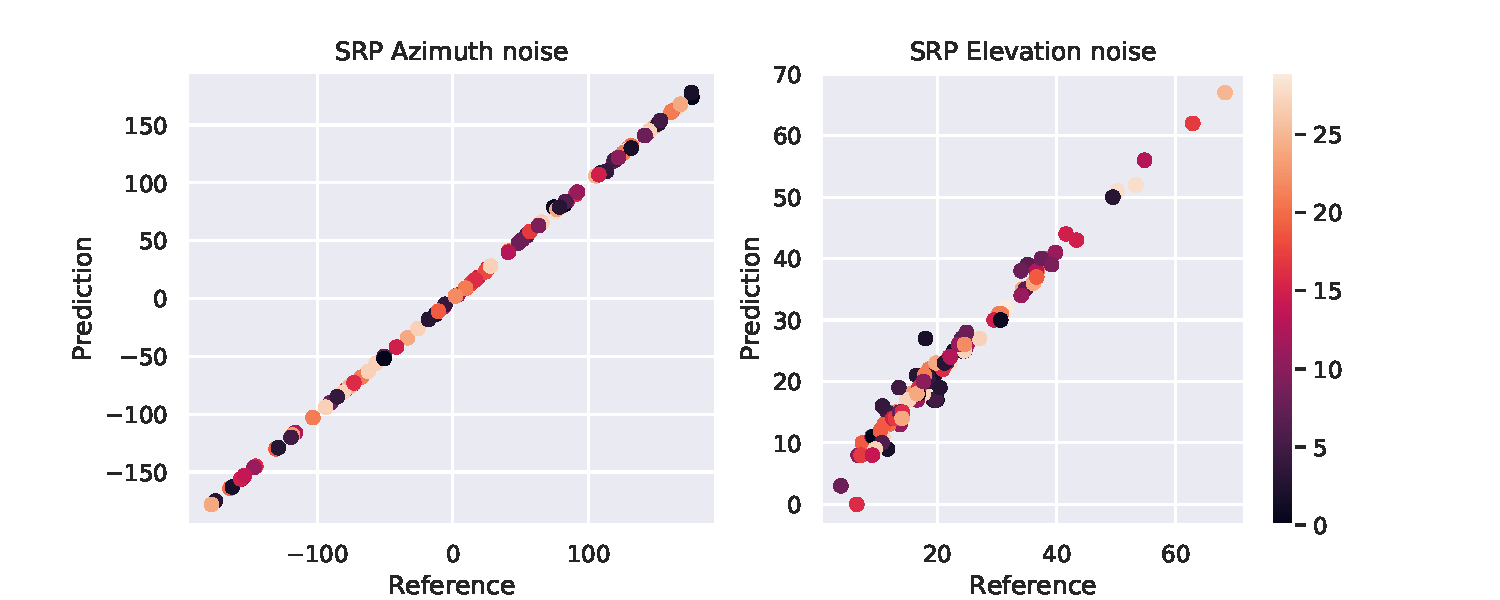
\includegraphics[width=\linewidth]{mirage/scatter_azel_estim_SRP_noise.pdf}
        \label{fig:mirage:synth_ssl_noise_srp}
    }
    \hfill
    \subfloat[azel_mirage][2D-SSL with  MIRAGE on noise data]{
        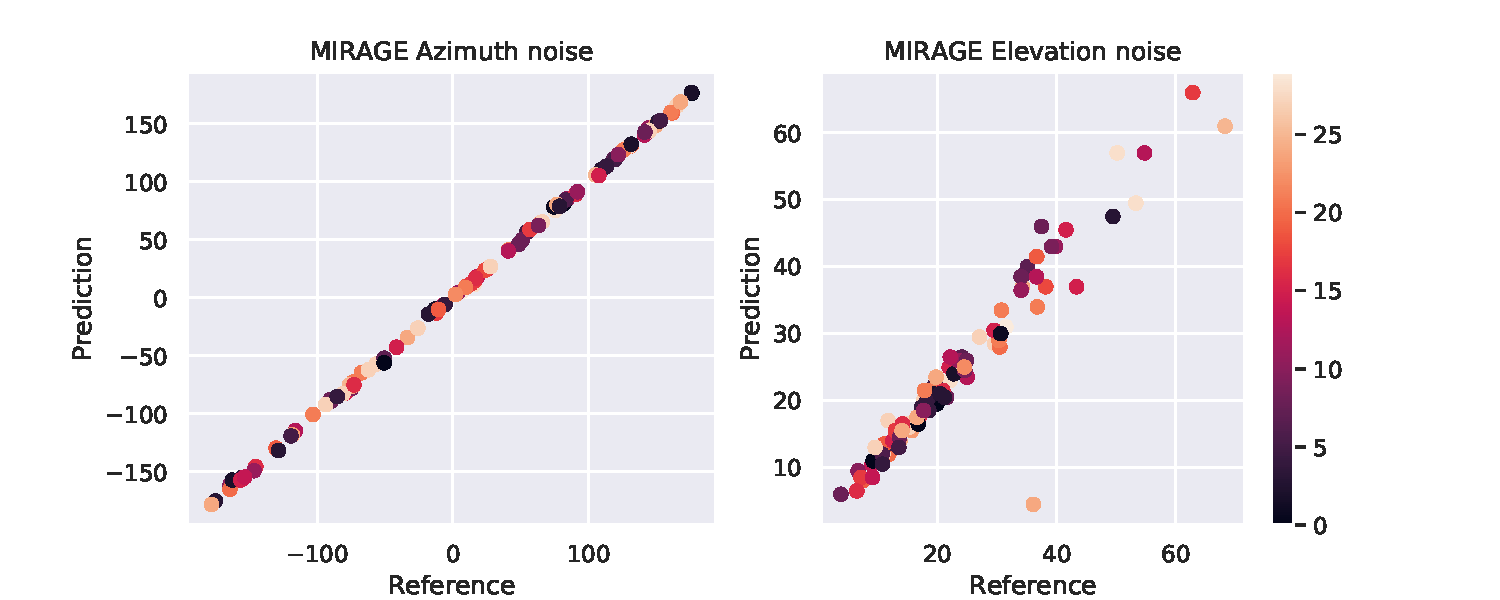
\includegraphics[width=\linewidth]{mirage/scatter_azel_estim_MIRAGE_noise.pdf}
        \label{fig:mirage:synth_ssl_noise_mirage}
    }
    \end{sidecaption}
\end{figure}

\begin{figure}[h]
    \begin{sidecaption}[]{
        Scatterplots (predictions-vs-ground-truth) for DoA estimation (azimuth and elevation) on synthetic data when the the source signal is \textbf{speech}.
        The color map corresponds to different SNR level [dB] in the data.
    }[fig:mirage:synth_ssl_speech]
    \centering
    \subfloat[azel_srp][2D-SSL with SRP-PHAT on speech data]{
        \centering
        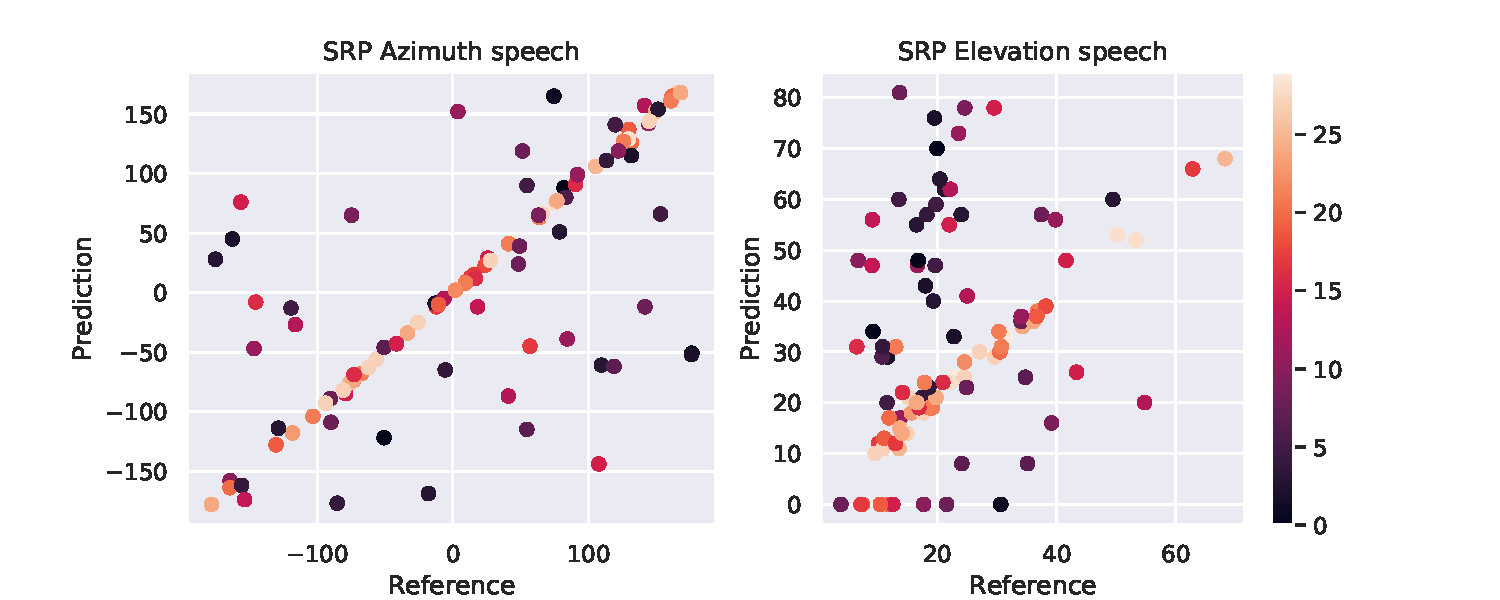
\includegraphics[width=\linewidth]{mirage/scatter_azel_estim_SRP_speech.pdf}
        \label{fig:mirage:synth_ssl_speech_srp}
    }
    \hfill
    \subfloat[azel_mirage][2D-SSL with  MIRAGE on speech data]{
        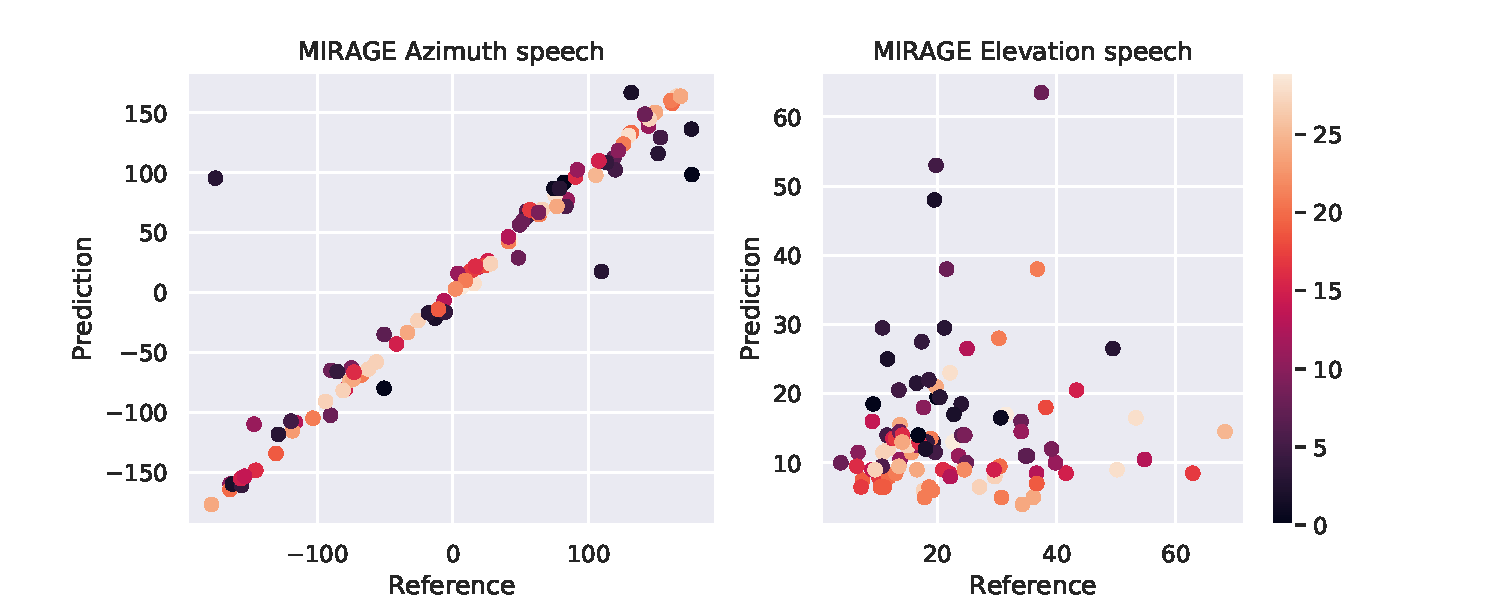
\includegraphics[width=\linewidth]{mirage/scatter_azel_estim_MIRAGE_speech.pdf}
        \label{fig:mirage:synth_ssl_speech}
    }
    \end{sidecaption}
\end{figure}

\subsection{Multi-channel real scenario}
\begin{figure}[t]
    \begin{fullwidth}
    \centering
    \subfloat[mu_spkr][Haru Array]{
        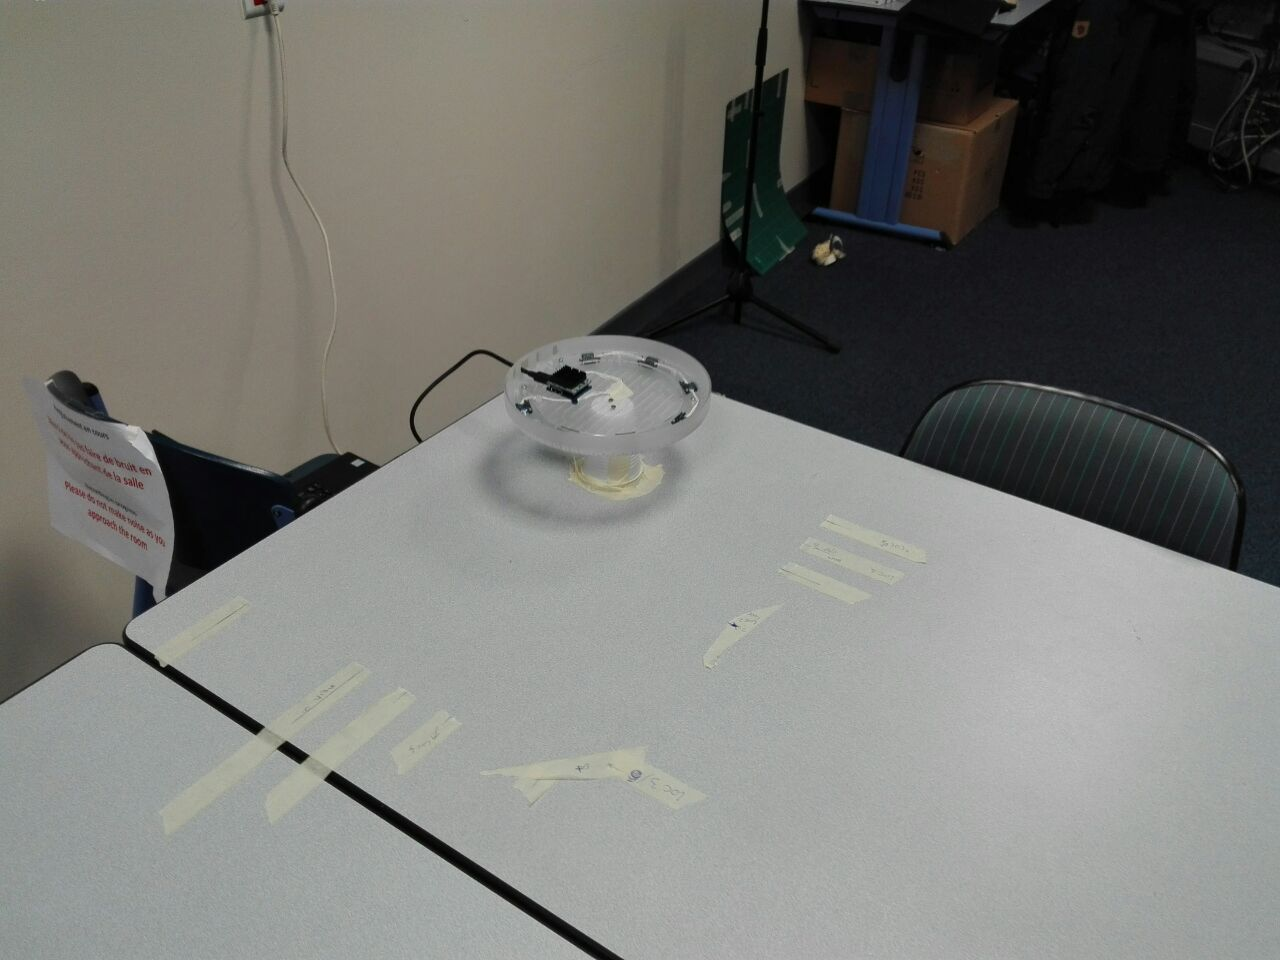
\includegraphics[width=0.32\textwidth]{figures/mirage/1_room_exp}}
    \hfill
    \subfloat[mu_spkr][Reflective table]{
        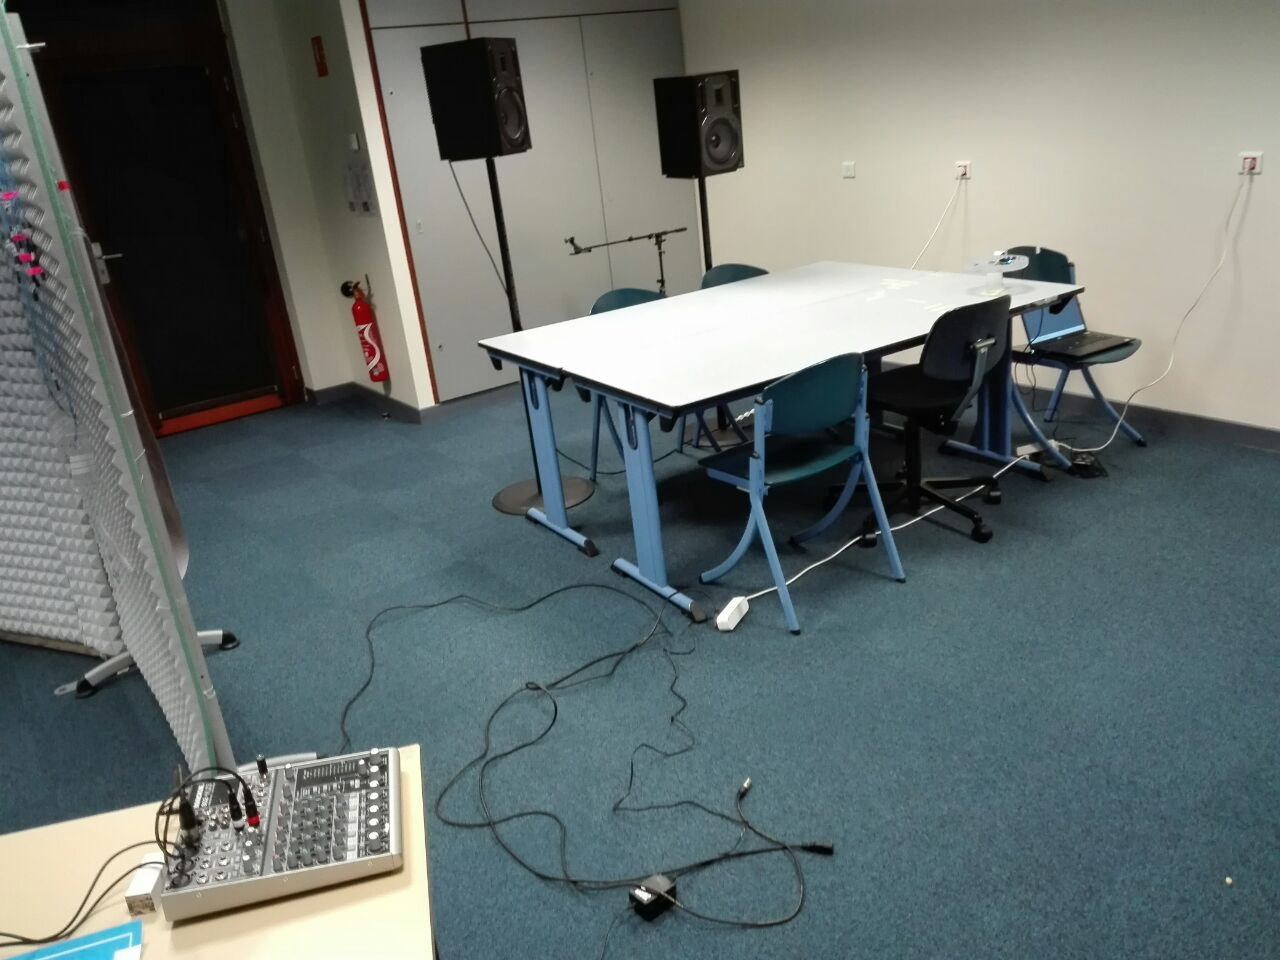
\includegraphics[width=0.32\textwidth]{figures/mirage/2_room_exp}}
    \hfill
    \subfloat[mu_univ][Detail]{
            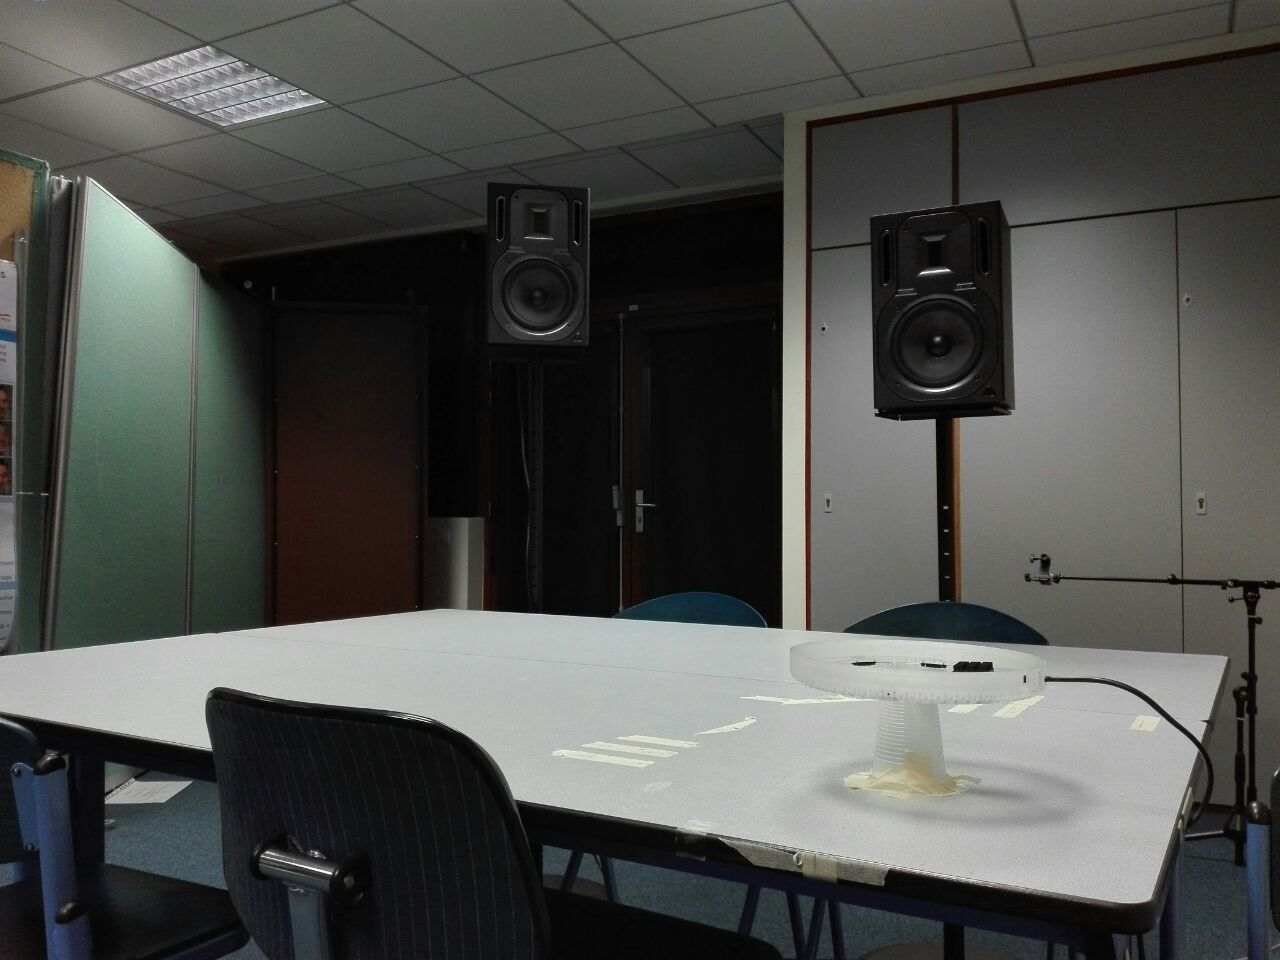
\includegraphics[width=0.32\textwidth]{figures/mirage/3_room_exp}}
    \label{fig:mirage:room_exp}
    \caption{Picture of the room and setup for recording real multichannel data with the HARU circular microphone array.}
    \end{fullwidth}
\end{figure}
In this section, we will analyze the two methods on real recordings.
The real multichannel data were recorded with the HONDA's HARU microphone circular array ($\numMics=7)$.
For the sake of simplicity, hereafter, we will denote this array as HARU.
The experiments were performed in a big office room 10~m $\times$ 15~m $\times$ 3~m with a reverberation time around 0.2 seconds.
The HARU was placed on top of a table with a height of 0.10 m to simulate the close-reflector scenario, used to train the \ac{DNN} model.
The room setup is shown in~\cref{fig:mirage:room_exp}.
Two loudspeakers were used the emit one anechoic and normalized utterance from the TIMIT dataset and 10 seconds of white noise.
The dataset consists in 5 different azimuthal positions and for each of them 2 different elevations yielding 10 different locations in space.
The geometry of the setup was annotated using metric tape measures.


\newthoughtpar{TDOA estimation and 2D-SSL performances on real data}
As reported in~\cref{tab:mirage:tdoa_real}, the two methods are comparable both for speech and noise emitted signals even if \ac{SRP-PHAT} performs slightly better.
In~\cref{fig:mirage:tdoa_real_pairs} the error on \ac{TDOA} estimation is shown of each microphone pair of the HARU.
It can be seen that the error and the deviation are not homogeneous among the pairs.
This might be due to some perturbations of the array's microphone positioning: the \ac{SRP-PHAT} method is only successful if the array's geometry is perfectly known \textit{a priori}.
However, little misplacement leads to local distortion in the input angular spectra\sidenote{
    In\citeonly{salvati2018exploiting}, the authors address this problem integrating \ac{SRP-PHAT} with a \ac{CNN} together.
}.
Moreover, the proposed approach needs the height of the robot (of each pair) as additional information, and again some perturbation can affect performances.

\begin{table}[h]
    \begin{sidecaption}[]{
        Evaluation metrics (\ac{nRMSE}, \ac{RMSE}, \ac{STD}) for TDOA estimation and empirical computational times for different source signals.
        Boldness denotes the best records.
    }[tab:mirage:tdoa_real]
    \centering
    \small
    \begin{tabular*}{\linewidth}{@{\extracolsep{\fill}}lllllll@{}}
        \toprule
        & &     signal &     nRMSE & RMSE &  STD &      time \\
        \midrule
        & MIRAGE  &       noise &  0.26 &  0.94 &  0.57 &  0.26 \\
        & SRP-PHAT &      noise &  0.20 &  0.62 &  0.57 &  6.48 \\
        \midrule
        & MIRAGE &       speech &  0.40 &  1.38 &  0.99 &  0.24 \\
        & SRP-PHAT &     speech &  0.32 &  0.82 &  1.08 &  4.02 \\
        \bottomrule
        \end{tabular*}
    \end{sidecaption}
\end{table}

\begin{figure}
    \begin{sidecaption}[]{
        Violin-plots of the TDOA estimation errors (in samples) versus the microphone pairs in HARU for two different source signals on real data
    }[fig:mirage:tdoa_real_pairs]
        \centering
        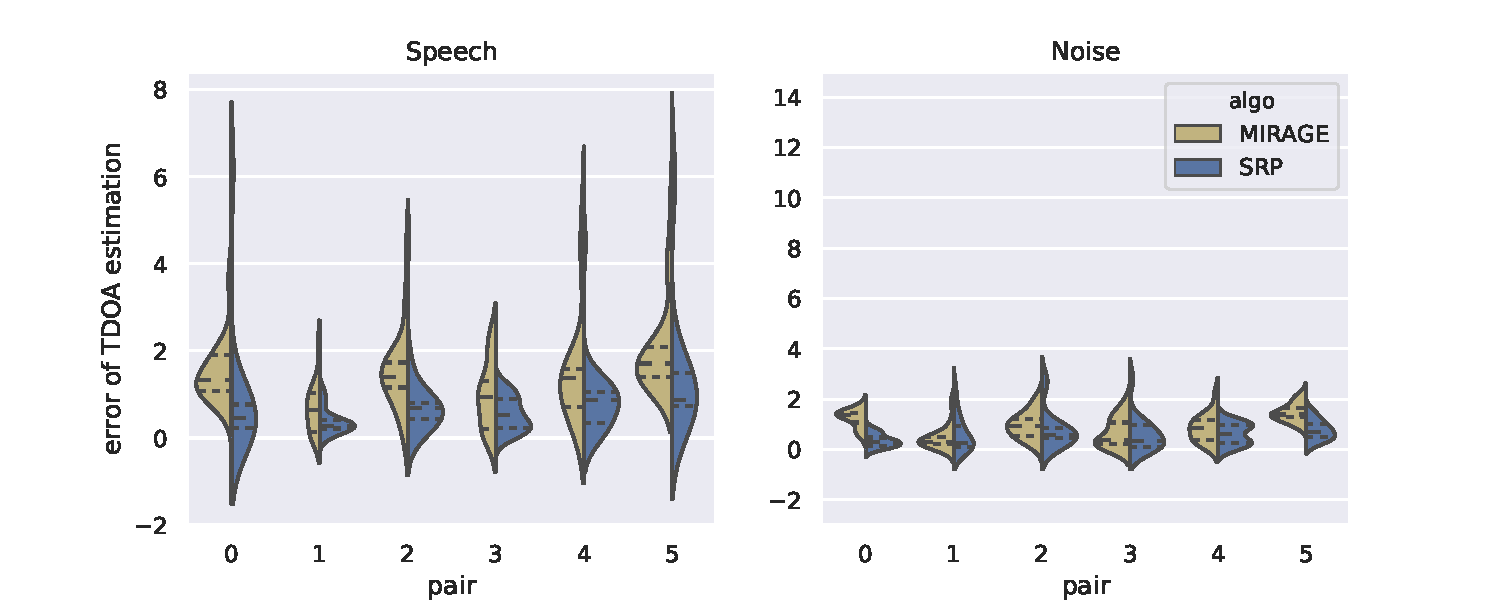
\includegraphics[trim={10 0 5 5},clip,width=\linewidth]{mirage/violinplot_tdoa_vs_pair_real.pdf}
    \end{sidecaption}
\end{figure}

\mynewline
Finally, we evaluate the performance of the methods for the 2D-\ac{SSL} task.
The results in terms of \ac{RMSE} and standard deviation are shown in~\cref{tab:mirage:ssl_real}.
When the signal emitted is speech, the CNN-based method outperforms the \ac{SRP-PHAT}.
However, the latter seems to perform better for noise signals, even if comparable error margins are observed.

\begin{table}[h]
    \begin{sidecaption}[]{
        Mean squared errors and standard deviations in degrees for estimation of azimuth ($\theta$) and elevation ($\phi$).
        In bold the best records.
    }[tab:mirage:ssl_real]
    \centering
    \small
    \begin{tabular*}{\linewidth}{@{\extracolsep{\fill}}lllll@{}}
        \toprule
        &          &  signal &  Error $\theta$  &  Error $\phi$ \\
        \midrule
        & MIRAGE   &   noise &   1.29 $\pm$   1.17 &     2.30 $\pm$  3.35 \\
        & SRP-PHAT &   noise &   \textbf{0.49 $\pm$   0.61} &     \textbf{1.70 $\pm$  1.42} \\
        \midrule
        & MIRAGE   &  speech & \textbf{  9.51 $\pm$  15.84} &    \textbf{12.26 $\pm$ 12.20} \\
        & SRP-PHAT &  speech &  35.27 $\pm$  54.57 &    15.10 $\pm$ 16.67 \\
        \bottomrule
    \end{tabular*}

    \end{sidecaption}
\end{table}

\mynewline
\Cref{fig:mirage:real_ssl_noise,fig:mirage:real_ssl_speech} illustrate the distribution of the prediction of the methods with respect to the ground-truth in the azimuth-vs-elevation planes.
We see that the predictions do not match the ground-truth properly.
SRP-PHAT seems to overestimate elevation while predicting well the azimuth, especially for noise signals.
MIRAGE seems to return more reasonable azimuth-elevation pairs.
However, the elevation prediction seems to be almost constant across the points.
Moreover, it seems that there is a constant offset or deviation, especially for azimuth prediction, suggesting that our real-data annotation was perhaps no accurate enough.

\begin{figure}[h]
    \begin{sidecaption}[]{
        Scatterplots (azimuth-vs-elevation) for DOA estimation on real data when the the source signal is \textbf{noise}.
        The colors indicate reference points (blue) and predicted ones (orange).
    }[fig:mirage:real_ssl_noise]
    \centering
    \subfloat[azel_srp][2D-SSL with SRP-PHAT on real noise data]{
        \centering
        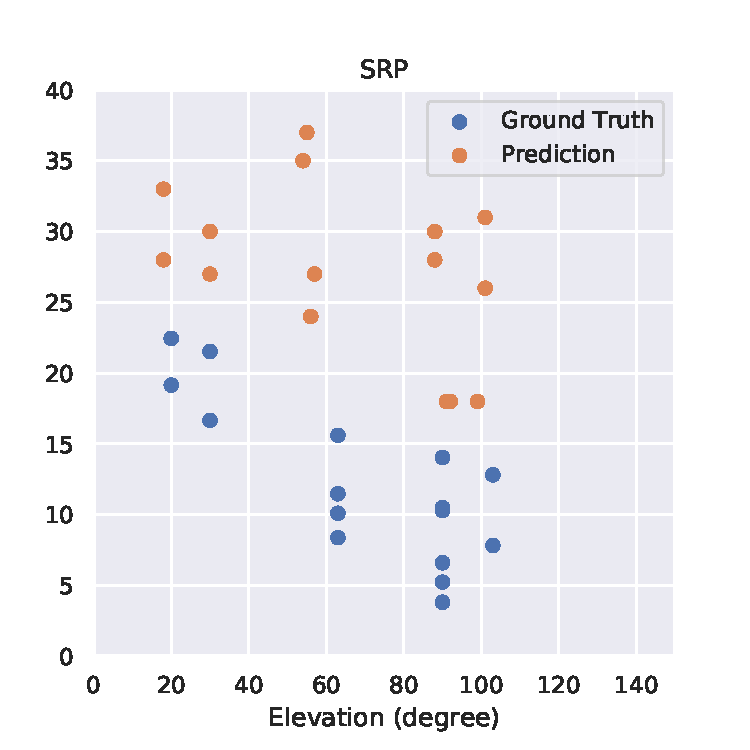
\includegraphics[width=0.47\linewidth]{mirage/scatterplot_SRP_broadband.pdf}
        \label{fig:mirage:real_ssl_noise_srp}
    }
    \hfill
    \subfloat[azel_mirage][2D-SSL with MIRAGE on real noise data]{
        \centering
        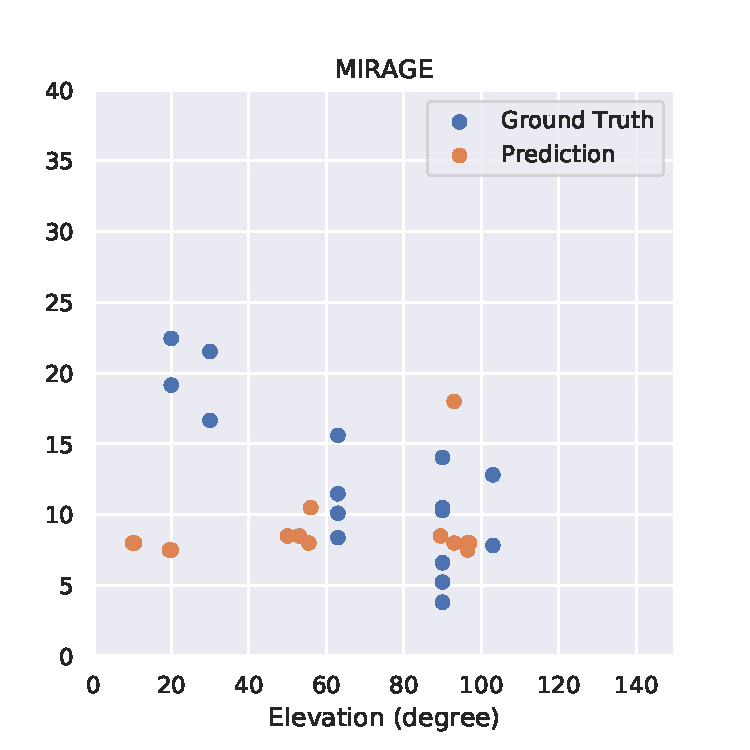
\includegraphics[width=0.47\linewidth]{mirage/scatterplot_MIRAGE_broadband.pdf}
        \label{fig:mirage:real_ssl_noise_mirage}
    }
    \end{sidecaption}
\end{figure}

\begin{figure}[h]
    \begin{sidecaption}[]{
        Scatterplots (azimuth-vs-elevation) for DoA estimation on real data when the source signal is \textbf{speech}.
        The colors indicate reference points (blue) and predicted ones (orange).
    }[fig:mirage:real_ssl_speech]
    \centering
    \subfloat[azel_srp][2D-SSL with SRP-PHAT on real noise data]{
        \centering
        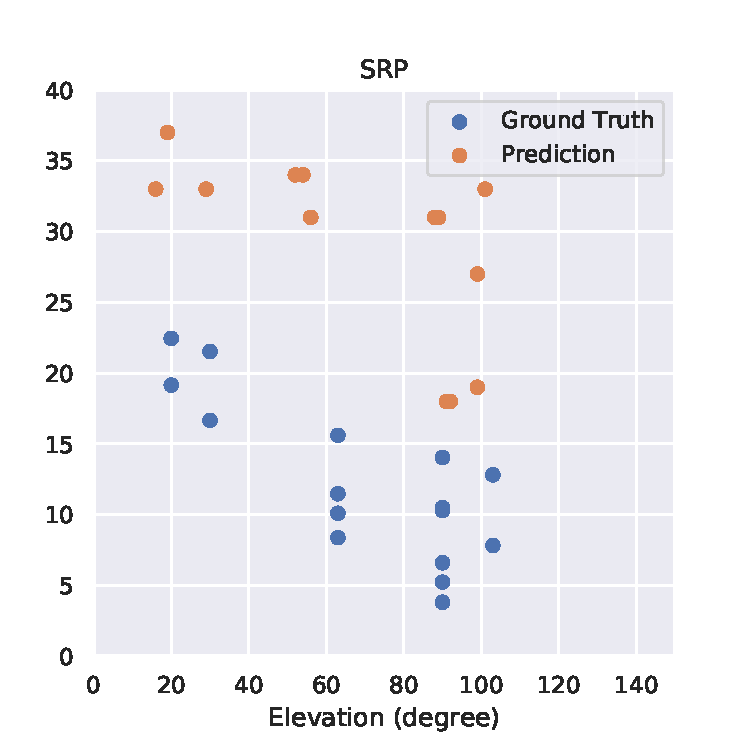
\includegraphics[width=0.47\linewidth]{mirage/scatterplot_SRP_speech.pdf}
        \label{fig:mirage:real_ssl_speech_srp}
    }
    \hfill
    \subfloat[azel_mirage][2D-SSL with MIRAGE on real noise data]{
        \centering
        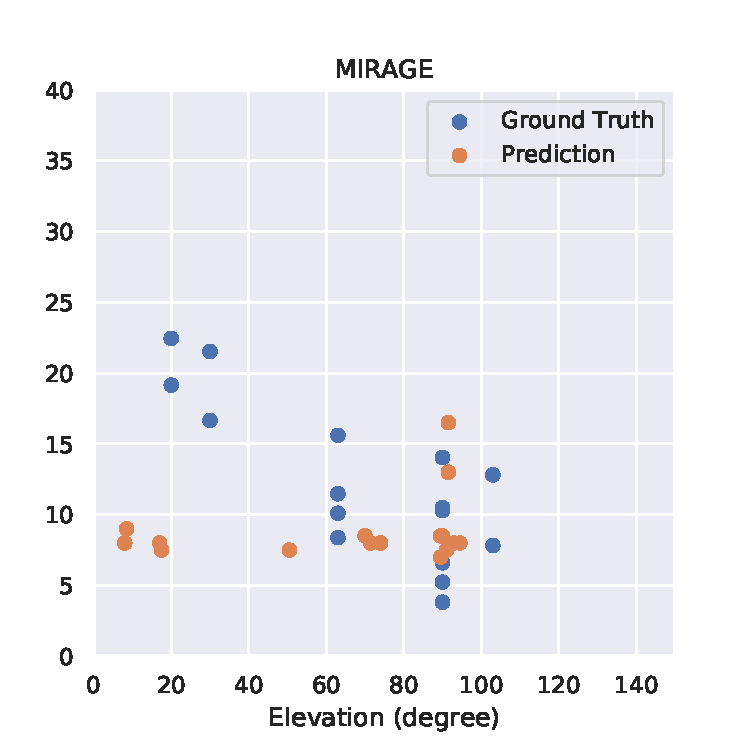
\includegraphics[width=0.47\linewidth]{mirage/scatterplot_MIRAGE_speech.pdf}
        \label{fig:mirage:real_ssl_speech_mirage}
    }
    \end{sidecaption}
\end{figure}


\section{Conclusion}
This chapter demonstrated how a simple echo model could boost an SSL algorithm in strongly echoic scenarios when microphones are placed close to a reflector.
Instead of integrating the physical equation into their algorithm, we proposed to use a successful algorithm for multichannel SSL on the virtual array created accounting for image microphone.
In order to create such an array, the echoes' parameters need to be estimated.
To this end, we use the learning-based acoustic echo retrieval methods proposed in~\cref{ch:lantern}.
\\Preliminary results on synthetic data for stereophonic recordings prove the effectiveness of the proposed approach.
However, results obtained on real data reveal that the task is still very challenging for both the proposed and baseline methods.
Considering the current knowledge, this is the first time an echo-aware method combines both knowledge-driven and data-driven for sound source localization.
The learning approach could still be significantly improved by considering other acoustic features (such as advance \ReTF/ methods), other architectures, and other challenges.
For instance, handling the missing frequencies of the speech while training on a broadband signal such as in~\citeonly{gaultier2017vast},
using physical-driven regulation such as in~\citeonly{nabian2020physics} and make the learning step independent to the array geometry.
Moreover, further investigation is needed to strengthen these results and further improve the robustness of the learned mapping, for which the \dEchorate may be used as a valuable testing dataset.